
\chapter{Hartree-Fock方法\label{chap:Hartree-Fock=0065B9=006CD5}}

\section{引言}

唯象壳模型的成功说明了核子确实是在一个所有核子形成的平均势中运动的。现在的问题是如何从如下两体相互作用中提取出这么一个单粒子势。

\[
V(1,\dots,A)=\sum^{A}_{i<j=1}V(i,j)\simeq\sum^{A}_{i=1}V(i)
\]

当然，从两体相互作用中提取出的单粒子势和到现在为止我们使用的单粒子势有何异同也是值得探究的。之后我们将会说明，通过把Slater行列式作为变分法的试探波函数，我们可以得到两体相互作用的单粒子势。

在\ref{sec:=0053D8=005206=00539F=007406}中，我们将会讨论普遍的变分原理——在接下来的章节中它势十分重要的。在\ref{sec:Hartree-Fock=0065B9=007A0B=007684=005BFC=0051FA}我们会详细讨论Hartree-Fock方法。在\ref{sec:=004E00=004E2A=0053EF=0089E3=006A21=00578B}我们会对一个非常简单的模型应用Hartree-Fock方法。在\ref{sec:Hartree-Fock=0065B9=006CD5=004E0E=005BF9=0079F0=006027}我们讨论了Hartree-Fock方法和对称性的关系，在\ref{sec:Hartree-Fock=0065B9=006CD5=004E0E=005BC6=005EA6=004F9D=008D56=0076F8=004E92=004F5C=007528}我们提出了密度依赖力的Hartree-Fock理论。

\section{变分原理\label{sec:=0053D8=005206=00539F=007406}}

Schrödinger方程为：
\begin{equation}
H|\Psi\rangle=E|\Psi\rangle\label{eq:schrodinger equation}
\end{equation}

它等价于变分法：
\[
\delta E[\Psi]=0
\]

这里：
\[
E[\Psi]=\frac{\langle\Psi|H|\Psi\rangle}{\langle\Psi|\Psi\rangle}
\]

由此得到：
\begin{equation}
\langle\delta\Psi|H-E|\Psi\rangle+\langle\Psi|H-E|\delta\Psi\rangle=0\label{eq:delta_E}
\end{equation}

由于一般来讲$|\Psi\rangle$是一个复数函数，我们可以对实部和虚部分别变分，这等价于对$|\delta\Psi\rangle$和$\langle\delta\Psi|$独立变分。为了看出这一点，我们利用\ref{eq:delta_E}对任意无穷小变换$|\delta\Psi\rangle$都成立。我们把$|\delta\Psi\rangle$替换为$\mathrm{i}|\delta\Psi\rangle$即可得到：
\[
-\mathrm{i}\langle\delta\Psi|H-E|\Psi\rangle+\mathrm{i}\langle\Psi|H-E|\delta\Psi\rangle
\]

同\ref{eq:delta_E}联立，我们即可发现：
\[
\langle\delta\Psi|H-E|\Psi\rangle=0
\]

当然我们同时还能发现这一方程的共轭。由于$|\delta\Psi\rangle$是任意的，上述方程就等价于本征值问题\ref{eq:schrodinger equation}。

变分法的近似来自于$|\Psi\rangle$被限制在一些简单的试探波函数组成的线性空间上。只要真实波函数没有在这个线性空间里，最小值解就不是真正的本征态，而仅仅是一个近似。变分法非常适合用来找到基态，因为对于任意试探波函数，我们可以有：
\begin{equation}
E[\Psi]\geq E_{0}\label{eq:variational principle for g.s.}
\end{equation}

因此$E_{0}$是变分计算的下确界。为了证明这一点，我们把试探波函数表示成一系列Hamilton量精确解的线性组合：
\[
|\Psi\rangle=\sum^{\infty}_{n=0}a_{n}|\Psi_{n}\rangle
\]

这里：
\[
H|\Psi_{n}\rangle=E_{n}|\Psi_{n}\rangle
\]

这导致：
\[
E[\Psi]=\frac{\sum_{nn^{\prime}}a^{*}_{n}a_{n}E_{n}\delta_{nn^{\prime}}}{\sum_{n}|a_{n}|^{2}}\geq\frac{\sum_{n}|a_{n}|^{2}E_{0}}{\sum_{n}|a_{n}|^{2}}=E_{0}
\]

这就证明了\ref{eq:variational principle for g.s.}。在基态能量非简并的情况下，当且仅当$n\neq0$的系数全部为零时，即$|\Psi\rangle$正比于$|\Psi_{0}\rangle$时，等号成立。如果我们对第一激发态感兴趣，我们就需要在正交于$|\Psi_{0}\rangle$的子空间内变分，也就是对所有$a_{0}=0$的波函数$|\Psi\rangle$变分。在这个子空间中，$|\Psi_{1}\rangle$的能量最小。为了得到$|\Psi_{1}\rangle$，我们要在$\langle\Psi_{1}|\Psi_{0}\rangle=0$的限制条件下变分。原则上我们可以像这样继续计算出整个能谱。

然而实际上，我们并不知道精确的$|\Psi_{0}\rangle$。由于我们是在一个Hilbert空间的子空间上做变分，因此只能得到一个近似的基态$|\Phi_{0}\rangle$。为了计算第一激发态$|\Psi_{1}\rangle$的近似$|\Phi_{1}\rangle$，我们必须在变分时加上$|\Phi_{1}\rangle$与$|\Phi_{0}\rangle$正交的条件：
\[
\langle\Phi_{1}|\Phi_{0}\rangle=0
\]

对于第二激发态，我们必须加上两个条件：
\[
\langle\Phi_{2}|\Phi_{1}\rangle=0\quad\text{和}\quad\langle\Phi_{2}|\Phi_{0}\rangle=0
\]

这些条件通过拉格朗日乘子法处理。可以看出，随着激发态越来越高，这一方法迅速变得非常复杂，因此这一方法主要用于处理基态。当然，有时由于对称性的存在这些条件非常容易满足，例如不同的态具有不同的角动量量子数的时候。我们将在\ref{chap:=0063A8=005E7F=007684=005355=007C92=005B50=006A21=00578B=00FF08HFB=007406=008BBA=00FF09}计算出整个转动谱——转动谱中所有的能级的计算都和基态一样简单。

我们已经证明，对于特定的试探波函数，由之计算出来的基态能量总是大于等于真实的基态能量，并且总是一个极值。除此之外我们还需要确定这个极值是极小值，为此我们需要计算能量泛函的二阶泛函导数，实际计算中就是对特定参数的二阶导。在Hartree-Fock或者Hartree-Fock-Bogoliubov理论\ref{chap:=0063A8=005E7F=007684=005355=007C92=005B50=006A21=00578B=00FF08HFB=007406=008BBA=00FF09}中，我们将要再次提到这一点。

为了确定哪一组试探波函数更好，我们有两个判断标准：
\begin{enumerate}
\item 如果某一组试探波函数是另一组的子集，那么更大的一组更好，因为它一定能得到另一组得到的极小值。
\item 由于精确的能量$E_{0}$是一个下界，我们期望两组试探波函数中得到的能量更低的一组更好。
\end{enumerate}
然而，这两个标准都不是绝对的。事实上可以找到一些违背这两个原则的例子。

最后，我们需要注意，变分原理仅仅对\ref{eq:schrodinger equation}这样的线性的本征值问题成立。在Hamilton量本身依赖于波函数时，我们必须非常小心。

\section{Hartree-Fock方程的导出\label{sec:Hartree-Fock=0065B9=007A0B=007684=005BFC=0051FA}}

\subsection{试探波函数的选取\label{subsec:=008BD5=0063A2=006CE2=0051FD=006570=007684=009009=0053D6}}

考虑到壳模型对原子核的很多性质都给出了定性的解释，我们可以假设存在一个平均单粒子势（Hartree-Fock势）：
\[
H^{\text{HF}}=\sum^{A}_{i=1}h(i)
\]

其能量最低的本征函数是真实基态波函数的一种近似。这一波函数$\Phi(1\dots A)$正如在\ref{chap:=0058F3=006A21=00578B}提到的，是Slater行列式：
\[
|\text{HF}\rangle=|\Phi(1\dots A)\rangle=\prod^{A}_{i=1}a^{\dagger}_{i}|\rangle
\]

这里费米算符$a^{\dagger}_{k}$，$a_{k}$是单粒子波函数$\varphi_{k}$对应的产生湮灭算符，它们本身就是单粒子Hamilton量$h$的本征函数：
\[
h(i)\varphi_{k}(i)=\varepsilon_{k}\varphi_{k}(i),\quad i=(\boldsymbol{r}_{i},s_{i},t_{i})
\]

正如我们在\ref{sec:=00591A=004F53=0095EE=009898=007684=0058F3=006A21=00578B=0065B9=006CD5}中看到的，如果我们让$|\text{HF}\rangle$占据了能量最低的$A$个单粒子能级，我们就可以得到最低的本征能量$H^{\text{HF}}$。接下来，我们用字幕$i,j$（空穴态）来表示$|\text{HF}\rangle$中的占据态，用$m,n$（粒子态）表示未占据态。如果我们没有区分是占据还是非占据，我们用$k,l,p,q$表示。

波函数$\varphi_{k}(\boldsymbol{r},s,t)$是单粒子Hamilton量$h$的本征态$|k\rangle$的坐标表象波函数。一般来讲，我们考虑的是一组任意正交完备的单粒子波函数$\{\chi_{l}\}$（例如球谐振子波函数）构成的组态空间。函数$\varphi_{k}$可以在这组基上展开：
\[
\varphi_{k}=\sum_{l}D_{lk}\chi_{l}
\]

如果我们对每一个波函数$\chi_{l}$都定义一个相应的费米产生湮灭算符$c^{\dagger}_{l}$，$c_{l}$，我们可以简单的把算符$a^{\dagger}_{k}$用$c^{\dagger}_{l}$表示：
\begin{equation}
a^{\dagger}_{k}=\sum_{l}D_{lk}c^{\dagger}_{l}\label{eq:transformation of create operator}
\end{equation}

由于$\{\varphi_{k}\}$和$\{\chi_{l}\}$都是正交完备的，变换矩阵$D$必须是酉的：
\begin{equation}
D^{\dagger}D=DD^{\dagger}=1\label{eq:unitary condition of D}
\end{equation}

这也保证了算符$(a^{\dagger}_{k},a_{k})$和$(c^{\dagger}_{l},c_{l})$都分别遵循费米对易关系。

正如在\ref{sec:Slater=00884C=005217=005F0F=007684=005355=007C92=005B50=005BC6=005EA6=0077E9=009635}中讨论的，Slater行列式$\Phi$和一组单粒子基$\varphi_{k}$之间没有一一对应的关系。任意不混合空穴态和粒子态的酉变换都不改变$\Phi$（至少在不考虑相位的意义上）。

因此，更方便的代表Slater行列式$|\Phi\rangle$的方式是用对应的单粒子密度矩阵：
\[
\rho_{ll^{\prime}}=\langle\Phi|c^{\dagger}_{l^{\prime}}c_{l}|\Phi\rangle
\]

从\ref{eq:transformation of create operator},\ref{eq:unitary condition of D}可以得到：
\[
\rho_{ll^{\prime}}=\sum_{kk^{\prime}}D_{lk}D^{*}_{l^{\prime}k^{\prime}}\langle\Phi|a^{\dagger}_{k^{\prime}}a_{k}|\Phi\rangle=\sum^{A}_{i=1}D_{li}D^{*}_{l^{\prime}i}
\]

这里第二个等号是因为$\rho$在$a^{\dagger}_{k}$，$a_{k}$这组基下是对角的，并且本征值对于空穴态是$1$，对于粒子态是$0$。$\rho$的迹恰好等于粒子数。

正如我们在\ref{sec:Slater=00884C=005217=005F0F=007684=005355=007C92=005B50=005BC6=005EA6=0077E9=009635}看到的，Slater行列式$\Phi$和单粒子密度矩阵$\rho$之间存在一一映射。Slater行列式的单粒子密度矩阵$\rho$可以通过他们的本征值是$0$或$1$来表征，也就是：
\[
\rho^{2}=\rho
\]

因此$\rho$就是单粒子波函数空间中投影到空穴态$\varphi_{i}$张成的子空间的投影算符。

同样的，我们可以定义投影算符$\sigma$：
\[
\sigma=1-\rho
\]

它投影到粒子态$\varphi_{m}$上。

Hartree-Fock方法可以如下定义：我们考虑有$A$个任意的正交单粒子波函数$\varphi_{i}$的Slater行列式组成的试探波函数集合，在这组集合上最小化能量。与之等价的陈述是我们考虑所有单粒子密度矩阵具有性质$\rho^{2}=\rho$和$\mathop{\text{Tr}}\rho=A$的波函数。

我们在接下来的章节中可以看到，这一变分过程能让我们得到单粒子算符$H^{\text{HF}}$
\begin{comment}
不是很确定能不能真得到，原文只说了有可能性。
\end{comment}
。

\subsection{Hartree-Fock能量}

在我们真正做变分以得到HF波函数之前，我们必须计算HF能量：
\[
E^{\text{HF}}=\langle\Phi|H|\Phi\rangle
\]

我们从多体Hamilton量$H$开始，把它用二次量子化的形式表示出来即有\ref{chap:=004E8C=006B21=0091CF=005B50=005316}：
\[
H=\sum_{l_{1}l_{2}}t_{l_{1}l_{2}}c^{\dagger}_{l_{1}}c_{l_{2}}+\frac{1}{4}\sum_{l_{1}l_{2}l_{3}l_{4}}\bar{v}_{l_{1}l_{2},l_{3}l_{4}}c^{\dagger}_{l_{1}}c^{\dagger}_{l_{2}}c_{l_{4}}c_{l_{3}}
\]

这里：
\[
\bar{v}_{l_{1}l_{2},l_{3}l_{4}}=v_{l_{1}l_{2}l_{3}l_{4}}-v_{l_{1}l_{2}l_{4}l_{3}}
\]

利用Wick定理，我们可以把能量表示为单粒子密度矩阵的泛函：
\begin{align}
E^{\text{HF}}[\rho] & =\sum_{l_{1}l_{2}}t_{l_{1}l_{2}}\langle\Phi|c^{\dagger}_{l_{1}}c_{l_{2}}|\Phi\rangle+\frac{1}{4}\sum_{l_{1}l_{2}l_{3}l_{4}}\bar{v}_{l_{1}l_{2}l_{3}l_{4}}\langle\Phi|c^{\dagger}_{l_{1}}c^{\dagger}_{l_{2}}c_{l_{4}}c_{l_{3}}|\Phi\rangle\nonumber \\
 & =\sum_{l_{1}l_{2}}t_{l_{1}l_{2}}\rho_{l_{2}l_{1}}+\frac{1}{2}\sum_{l_{1}l_{2}l_{3}l_{4}}\rho_{l_{3}l_{1}}\bar{v}_{l_{1}l_{2}l_{3}l_{4}}\rho_{l_{4}l_{2}}\label{eq:HF energy}\\
 & =\mathop{\text{Tr}}(t\rho)+\frac{1}{2}\mathop{\text{Tr}}_{1}\mathop{\text{Tr}}_{1}(\rho\bar{v}\rho)\nonumber 
\end{align}

这里$\mathop{\text{Tr}}_{1}\mathop{\text{Tr}}_{1}\dots$是一个偷懒的记号。这一个式子与基的选择无关，因此我们可以取一组HF基$\{\varphi_{k}\}$，此时$\rho$是对角的，对角元是$0$或者$1$，因此HF能量为：
\begin{equation}
E^{\text{HF}}=\sum^{A}_{i=1}t_{ii}+\frac{1}{2}\sum^{A}_{i,j=1}\bar{v}_{ij,ij}\label{eq:HF energy in HF basis}
\end{equation}


\subsection{对能量的变分}

为了确定HF基，我们必须在波函数是直积波函数$|\Phi\rangle$的情况下，或者说在单粒子密度矩阵$\rho$具有性质$\rho^{2}=\rho$的情况下，使能量最小。由于$\rho$的变分$\rho+\delta\rho$必须仍然是一个投影算符，因此我们有：
\[
(\rho+\delta\rho)^{2}=\rho+\delta\rho
\]

展开到$\delta\rho$的线性项，有：
\[
\delta\rho=\rho\,\delta\rho+\delta\rho\,\rho
\]

上式意味着在HF基下粒子粒子（pp）和空穴空穴（hh）矩阵元必须为零，也就是说
\begin{comment}
左乘$\rho$即可得到$\rho\,\delta\rho\,\rho=0$，或者移项得到$\sigma\,\delta\rho=\delta\rho\,\rho$，右乘$\sigma$得到$\sigma\,\delta\rho\,\sigma=0$。
\end{comment}
：
\[
\rho\,\delta\rho\,\rho=\sigma\,\delta\rho\,\sigma=0
\]

在试探波函数为Slater行列式的情况下，为了确保这一点，我们只可以对HF基下的ph和hp矩阵元做变分$\delta\rho_{mi}$和$\delta\rho_{im}$
\begin{comment}
这里非常令人迷惑，实际上，只有在HF基下ph矩阵元和hp矩阵元才是零，其它基下并不如此，但是HF基是我们求解得到的，并不是提前就知晓的，因此我们并不知道HF基下的ph和hp矩阵元到底是什么。所以这里的推导只是形式上的推导，得到的是已知HF基后需要满足的条件。
\end{comment}
。

能量的变分因此为：
\begin{equation}
\delta E=E[\rho+\delta\rho]-E[\rho]=\sum_{kk^{\prime}}h_{kk^{\prime}}\delta\rho_{k^{\prime}k}=\sum_{mi}h_{mi}\delta\rho_{im}+\text{c.c.}\label{eq:variation of energy}
\end{equation}

这里厄米矩阵$h$的定义为：
\[
h_{kk^{\prime}}=\frac{\partial E^{\text{HF}}[\rho]}{\partial\rho_{k^{\prime}k}}
\]

从\ref{eq:HF energy}我们可以得到：
\[
h=t+\Gamma
\]

这里自洽场$\Gamma$为：
\[
\Gamma_{kk^{\prime}}=\sum_{ll^{\prime}}\bar{v}_{kl^{\prime}k^{\prime}l}\rho_{ll^{\prime}}
\]

由于$\delta\rho_{mi}$的任意值都是允许的，我们从\ref{eq:variation of energy}可以看出，变分$\delta E=0$实际上就是说$h$的ph矩阵元必须为零：
\[
h_{mi}=t_{mi}+\sum^{A}_{j=1}\bar{v}_{mjij}=0\quad(i\leq A,m>A)
\]

在HF基下，$\rho$是对角的，此时$h$不会把$\rho$的粒子态和空穴态混合，因此上式等价于：
\[
[h,\rho]=[t+\Gamma[\rho],\rho]=0
\]

\begin{booknote*}
考虑此时具体的矩阵形式，写成分块矩阵即为：
\[
\rho=\begin{bmatrix}1 & 0\\
0 & 0
\end{bmatrix},h=\begin{bmatrix}a & 0\\
0 & b
\end{bmatrix}
\]

此时显然有：
\[
[h,\rho]=\begin{bmatrix}a & 0\\
0 & b
\end{bmatrix}\begin{bmatrix}1 & 0\\
0 & 0
\end{bmatrix}-\begin{bmatrix}1 & 0\\
0 & 0
\end{bmatrix}\begin{bmatrix}a & 0\\
0 & b
\end{bmatrix}=0
\]
\end{booknote*}
这是一个非线性方程，求解十分困难。上式也是在说$h$和$\rho$可以同时对角化。由于对于粒子态之间的酉变换或者空穴态之间的酉变换$\rho$是对角的这一条件仍然能得到满足，因此我们可以利用这一自由度来让$h$也变成对角的。这决定了Hartree-Fock基，并且把上述方程变成了一个本征值问题：
\begin{equation}
h_{kk^{\prime}}=t_{kk^{\prime}}+\sum^{A}_{i=1}\bar{v}_{kik^{\prime}i}=\varepsilon_{k}\delta_{kk^{\prime}}\label{eq:single particle hamiltonian}
\end{equation}

考虑到这一组基是通过变换$D$\ref{eq:transformation of create operator}得到的，我们可以得到Hartree-Fock方程集
\begin{comment}
神他妈Hartree-Fock方程集（the set of Hartree-Fock equations）。不过这里啰哩啰唆的好像读者都不知道什么是本征值问题一样。
\end{comment}
：
\[
\sum_{l^{\prime}}h_{ll^{\prime}}D_{l^{\prime}k}=\sum_{l^{\prime}}\left(t_{ll^{\prime}}+\sum^{A}_{i=1}\sum_{pp^{\prime}}\bar{v}_{lp^{\prime}l^{\prime}p}D_{pi}D^{*}_{p^{\prime}i}\right)D_{l^{\prime}k}=\varepsilon_{k}D_{lk}
\]

这表示一个厄米本征值问题。它是非线性的，因为矩阵$h$依赖于密度矩阵$\rho$，也就是说，这个问题的解。可以从这些方程确定的系数矩阵$D_{lk}$中得到波函数$\varphi_{k}$。

我们因此可以得到一个单粒子Hamilton量：
\begin{align*}
H^{\text{HF}} & =\sum_{kk^{\prime}}h_{kk^{\prime}}a^{\dagger}_{k}a_{k^{\prime}}=\sum_{kk^{\prime}}(t+\Gamma)_{kk^{\prime}}a^{\dagger}_{k}a_{k^{\prime}}\\
 & =\sum_{kk^{\prime}}\left(t_{kk^{\prime}}+\sum^{A}_{j=1}\bar{v}_{kjk^{\prime}j}\right)a^{\dagger}_{k}a_{k^{\prime}}=\sum_{k}\varepsilon_{k}a^{\dagger}_{k}a_{k}
\end{align*}

它拥有\ref{subsec:=008BD5=0063A2=006CE2=0051FD=006570=007684=009009=0053D6}中提到的性质。它对应基态就是Slater行列式$|\text{HF}\rangle$，最底的$A$个能级是占据的，其对应的能量在波函数的变分下是稳定的
\begin{comment}
我估计作者自己都不知道自己在写什么。
\end{comment}
。

单粒子Hamilton量$h$除了动能$t$外，还包含一个自洽场$\Gamma$，它依赖于原子核的密度。它是对所有的两体相互作用平均后的单粒子场。这在坐标空间会更清晰\ref{subsec:=005750=006807=007A7A=0095F4=007684Hartree-Fock=0065B9=007A0B}。HF波函数$|\text{HF}\rangle$的能量期待值可以由\ref{eq:HF energy in HF basis}和\ref{eq:single particle hamiltonian}给出：
\[
E^{\text{HF}}_{0}=\sum^{A}_{i=1}\varepsilon_{i}-\frac{1}{2}\sum^{A}_{ij=1}\bar{v}_{ijij}
\]

因此它并不等于所有单粒子能量之和。

\subsection{坐标空间的Hartree-Fock方程\label{subsec:=005750=006807=007A7A=0095F4=007684Hartree-Fock=0065B9=007A0B}}

为了更好的理解Hartree-Fock方程，我们把它在坐标空间写出来。我们这里假设两体相互作用不依赖于自旋或者同位旋，也就是一个纯的Wigner力\ref{sec:=0088F8=006838=00529B}。我们可以得到：
\[
-\frac{\hbar^{2}}{2m}\nabla^{2}\varphi_{k}(\boldsymbol{r})+\sum^{A}_{j=1}\int\mathrm{d}\boldsymbol{r}^{\prime}\,v(\boldsymbol{r},\boldsymbol{r}^{\prime})\cdot\varphi^{*}_{j}(\boldsymbol{r}^{\prime})\left(\varphi_{j}(\boldsymbol{r}^{\prime})\varphi_{k}(\boldsymbol{r})-\varphi_{j}(\boldsymbol{r})\varphi_{k}(\boldsymbol{r}^{\prime})\right)=\varepsilon_{k}\varphi_{k}(\boldsymbol{r})
\]

定义Hartree势：
\[
\Gamma_{\text{H}}(\boldsymbol{r})=\int\mathrm{d}\boldsymbol{r}^{\prime}\,v(\boldsymbol{r},\boldsymbol{r}^{\prime})\sum^{A}_{j=1}\left|\varphi_{j}(\boldsymbol{r}^{\prime})\right|^{2}=\int\mathrm{d}\boldsymbol{r}^{\prime}\,v(\boldsymbol{r},\boldsymbol{r}^{\prime})\rho(\boldsymbol{r}^{\prime})
\]

和非局域的交换势：
\[
\Gamma_{\text{Ex}}(\boldsymbol{r},\boldsymbol{r}^{\prime})=-v(\boldsymbol{r},\boldsymbol{r}^{\prime})\sum^{A}_{j=1}\varphi^{*}_{j}(\boldsymbol{r}^{\prime})\varphi_{j}(\boldsymbol{r})=-v(\boldsymbol{r},\boldsymbol{r}^{\prime})\rho(\boldsymbol{r},\boldsymbol{r}^{\prime})
\]

我们发现$\varphi_{k}(\boldsymbol{r})$是一个非局域Schr\"odinger方程的解：
\[
\left(-\frac{\hbar^{2}}{2m}\nabla^{2}+\Gamma_{\text{H}}(\boldsymbol{r})\right)\varphi_{k}(\boldsymbol{r})+\int\mathrm{d}\boldsymbol{r}^{\prime}\,\Gamma_{\text{Ex}}(\boldsymbol{r},\boldsymbol{r}^{\prime})\varphi_{k}(\boldsymbol{r},\boldsymbol{r}^{\prime})=\varepsilon_{k}\varphi_{k}(\boldsymbol{r})
\]

上述方程是一个自洽问题，因为势$\Gamma,\Gamma_{\text{H}},\Gamma_{\text{Ex}}$依赖于局域或者非局域的势$\rho(\boldsymbol{r})$和$\rho(\boldsymbol{r},\boldsymbol{r}^{\prime})$。这些方程可以通过迭代求解，迭代第一步可以从一组唯象的壳模型波函数出发，计算$\Gamma_{\text{H}}$和$\Gamma_{\text{Ex}}$，也可以从Thomas-Fermi近似得到的密度出发。从上述表达式，我们可以进一步得到新的单粒子波函数等等。这一步骤持续进行直到收敛，也就是两次迭代间势能不再变化。在这种情况下，$\Gamma$是单个粒子在其它粒子组成的背景下感受到的自洽单粒子平均势。

需要强调的是，从一个局域的两体相互作用出发，我们得到的Fock势$\Gamma_{\text{Ex}}$也是非局域的。这是因为Pauli不相容原理和矩阵元的反对称化。对一个简单的没有反对称化的直积波函数做变分只会得到Hartree势。当然，非局域的两体相互作用会导致Hartree势也是非局域的。另一个角度来说，如果我们使用$\delta$力，那么Fock项也是局域的。

由于更多关于HF理论的框架的讨论会在\ref{chap:=0063A8=005E7F=007684=005355=007C92=005B50=006A21=00578B=00FF08HFB=007406=008BBA=00FF09}中给出，因此我们这里不再深入讨论各种细节。我们仅仅在这里讨论Hartree-Fock方程的稳定线，也就是说，Hartree-Fock方程的解是对应能量的极大值还是极小值。我们也会展示一种叫做梯度法的HF方程求解方式。

为了使读者熟悉这一章中提到的概念，我们现在展示一个简单的模型，它对应的HF方程可以完全解析的求解。

\section{一个可解模型\label{sec:=004E00=004E2A=0053EF=0089E3=006A21=00578B}\label{sec:5.4_Lipkin=006A21=00578B}}

正如我们在上一节所讨论的，所有真实的HF方程求解都是非常复杂的数值问题。为了深入了解这一方法是如何工作的，我们把它应用到一个非常简单的、严格可解的模型中去。这一模型最初由Lipkin、Meshkov和Glick提出\cite{LMG65}，并且已经被广泛用于许多多体理论的检验（正如我们后续所见）。让我们设想一个固定的核芯单粒子势，它由其余核子构成特别稳定的核芯所产生。此时可以近似认为，平均势中仅来自最后一个$j$-壳层中核子的那一部分可以通过自洽方式求解，而忽略核芯与最后一个$j$-壳层的相互影响。当然，在费米面之上仅存在一个具有相同$j$的单粒子能级的设想是不实际的，其目的仅在于将问题图式化。

此外，假定在由核芯固定势产生的基底中，两个壳层内核子的剩余相互作用具有非常特殊的形式：它是单极-单极（monopole-monopole）类型的（见第4章），且本质上仅有一个非零矩阵元（RPA类型的粒子-空穴矩阵元，见第8章）。该模型的Hamilton量具有如下形式：

\begin{equation}
H=\epsilon K_{0}-\frac{1}{2}V\left(K^{2}_{+}+K^{2}_{-}\right)\label{eq:5.45}
\end{equation}
其中

\begin{equation}
K_{0}=\frac{1}{2}\sum^{\Omega}_{m=1}\left(c^{\dagger}_{1m}c_{1m}-c^{\dagger}_{-1m}c_{-1m}\right),\quad K_{+}=\sum^{\Omega}_{m=1}c^{\dagger}_{1m}c_{-1m},\quad K_{-}=\left(K_{+}\right)^{\dagger}\label{eq:5.46}
\end{equation}
这里$\Omega=2j+1$，算符$c^{\dagger}_{1m}$与$c^{\dagger}_{-1m}$分别在上下两个能级上产生一个粒子，而$\epsilon$为两能级之间的能量差（见\ref{fig:5_1}）。算符$K_{0},K_{\pm}$满足角动量的对易关系：

\begin{equation}
\left[K_{+},K_{-}\right]=2K_{0},\quad\left[K_{0},K_{\pm}\right]=\pm K_{\pm}\label{eq:5.47}
\end{equation}

\begin{figure}[H]
\begin{centering}
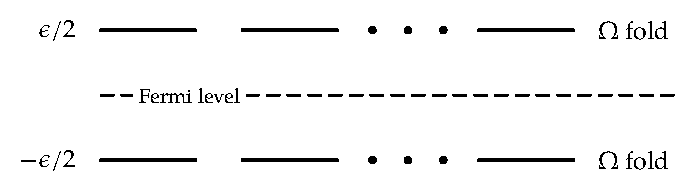
\includegraphics[width=0.75\textwidth]{pictures/5_1}
\par\end{centering}
\caption{\label{fig:5_1}示意模型中的能级结构（两能级相距$\epsilon$，各具$\Omega$重简并，其间为费米面）。}
\end{figure}

然而必须强调的是，算符$K_{0},K_{\pm}$与坐标空间中的转动毫无关系，它们通常被称为准自旋（quasi-spin）算符。为了应用Hartree-Fock方法，我们需要构建一般的Slater行列式$|\Phi\rangle$。Hamilton量\ref{eq:5.45}在费米面下方$\Omega$个能级与费米面上方相应能级之间的置换下保持不变。因此，在下文中我们局限于对这种置换完全对称的解。在这种情况下，仅存在一种激发粒子-空穴对的可能，最一般的Slater行列式$|\Phi\rangle$由复数$z$表征：

\begin{equation}
|\Phi\rangle=\mathcal{N}\exp\left(zK_{+}\right)|\Phi_{0}\rangle=\prod^{\Omega}_{m=1}a^{\dagger}_{0m}|-\rangle\label{eq:5.48}
\end{equation}
其中

\begin{equation}
|\Phi_{0}\rangle=\prod^{\Omega}_{m=1}c^{\dagger}_{-1m}|-\rangle\label{eq:5.49}
\end{equation}
且

\begin{align}
a^{\dagger}_{0m} & =D_{-0}c^{\dagger}_{-1m}+D_{+0}c^{\dagger}_{1m}\label{eq:5.50a}\\
a^{\dagger}_{1m} & =D_{-1}c^{\dagger}_{-1m}+D_{+1}c^{\dagger}_{1m}\label{eq:5.50b}
\end{align}
这里我们将新的上下能级分别记为0和1。借助式\ref{eq:5.50a}与\ref{eq:5.50b}，我们可以用新算符$a_{0m},a_{1m}$表示Hamilton量\ref{eq:5.45}。随后，在$D$归一化条件（$|D_{-0}|^{2}+|D_{+0}|^{2}=1$）下对$\langle\Phi|H|\Phi\rangle$关于$D_{\pm0}$变分，即可导出Lipkin模型中的Hartree-Fock方程：

\begin{equation}
\begin{pmatrix}-\frac{1}{2}\epsilon & -Q\\
-Q^{*} & \frac{1}{2}\epsilon
\end{pmatrix}\begin{pmatrix}D_{-0}\\
D_{+0}
\end{pmatrix}=\epsilon_{0}\begin{pmatrix}D_{-0}\\
D_{+0}
\end{pmatrix}\label{eq:5.51}
\end{equation}
其中

\begin{equation}
\chi=\frac{V(\Omega-1)}{\epsilon},\quad Q=\chi\epsilon D_{+0}D^{*}_{-0}
\end{equation}
这是通常的非线性方程，可通过迭代法求解。新的单粒子能量由下式给出：

\begin{equation}
\epsilon_{0,1}=\mp\frac{1}{2}\epsilon\sqrt{1+\left(\frac{2|Q|}{\epsilon}\right)^{2}}=\mp\frac{1}{2}\epsilon\sqrt{1+\chi^{2}\sin^{2}2\alpha}\label{eq:5.52}
\end{equation}
其中我们令$D_{-0}=\cos\alpha$，$D_{+0}=\sin\alpha\,\mathrm{e}^{-\mathrm{i}\varphi}$。由式\ref{eq:5.51}解出$D_{-0},D_{+0}$并代入$Q$的表达式，在$Q\neq0$的情形下，利用式\ref{eq:5.52}可得关于“形变”势$Q$的如下方程：

\begin{equation}
1=\frac{\chi}{\sqrt{1+\left(\frac{2|Q|}{\epsilon}\right)^{2}}}\label{eq:5.53}
\end{equation}
该方程仅在$\chi\ge1$时具有实数解，对应于下文给出的形变HF解。（式\ref{eq:5.53}与BCS理论的能隙方程极其相似，这绝非偶然，我们在第11.2节与附录F.5中将对此进行更为详尽的讨论。）

在坐标$\alpha,\varphi$下，基态能量表示为

\begin{equation}
E_{\mathrm{HF}}=-\frac{1}{2}\epsilon\Omega\left(\cos2\alpha+\frac{1}{2}\chi\sin^{2}2\alpha\cos2\varphi\right)\label{eq:5.54}
\end{equation}
自洽条件由能量对参数的极值给出：

\begin{align}
\frac{\partial E_{\mathrm{HF}}}{\partial\alpha} & =0=\epsilon\Omega\sin2\alpha\left(1-\chi\cos2\alpha\cos2\varphi\right)\label{eq:5.55}\\
\frac{\partial E_{\mathrm{HF}}}{\partial\varphi} & =0=\frac{1}{2}\epsilon\Omega\chi\sin^{2}2\alpha\sin2\varphi\nonumber 
\end{align}
从式\ref{eq:5.55}可以看出，根据$\chi$大于还是小于1，必须区分两种情况。在后一种情形（$\chi<1$）下，仅有一个解：

\begin{equation}
\varphi_{\mathrm{HF}}=0,\quad\alpha_{\mathrm{HF}}=0\quad(\chi<1)\label{eq:5.56}
\end{equation}
对于$\chi>1$，存在第二个解：

\begin{equation}
\varphi_{\mathrm{HF}}=0,\quad\chi\cos2\alpha_{\mathrm{HF}}=1\quad(\chi>1)\label{eq:5.57}
\end{equation}
可以证明该解对应能量的极小值，而第一个解变为极大值。这可以从该点处能量曲面的曲率看出：

\begin{equation}
\left.\frac{\partial^{2}E_{\mathrm{HF}}}{\partial\alpha^{2}}\right|_{\alpha_{\mathrm{HF}}}=2\epsilon\Omega\left(\chi-\frac{1}{\chi}\right)>0\quad(\chi>1)\label{eq:5.58}
\end{equation}
在\ref{fig:5_2}中，我们给出了$\chi\lessgtr1$时二维能量曲面（式\ref{eq:5.54}）沿$\varphi=0$的剖面线。

\begin{figure}[H]
\begin{centering}
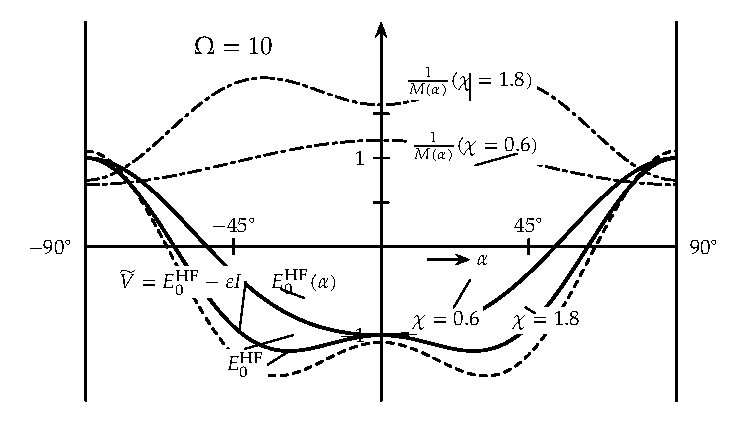
\includegraphics[width=0.75\textwidth]{pictures/5_2}
\par\end{centering}
\caption{\label{fig:5_2}$\chi\lessgtr1$时$E_{\mathrm{HF}}$作为$\alpha$的函数（实线）。其他四条曲线对应于生成坐标法（GCM，见第10.7.5小节）计算的量（引自\cite{Ho73}）。}
\end{figure}

从临界相互作用强度

\begin{equation}
\chi_{c}=\frac{V_{c}(\Omega-1)}{\epsilon}=1\label{eq:5.59}
\end{equation}
开始，位于$\alpha=0,\varphi=0$处的球形解变得不稳定，此时必须采用新的单粒子基底。在\ref{fig:5_3}中，展示了$\chi=6$时方程\ref{eq:5.51}的迭代求解过程。若从初值$\alpha_{1}=80^{\circ},\varphi_{1}=30^{\circ}$出发，后续各步依次为（\ref{fig:5_3}中的实线）：$\alpha_{2}=32.01^{\circ},\varphi_{2}=-30^{\circ}$；$\alpha_{3}=39.75^{\circ},\varphi_{3}=30^{\circ}$；$\alpha_{4}=40.19^{\circ},\varphi_{4}=-30^{\circ}$；……关于变量$\alpha$，解迅速收敛到$\alpha_{\mathrm{HF}}=40.20^{\circ}$（式\ref{eq:5.57}）；但关于变量$\varphi$，迭代解并未收敛，而是在$+30^{\circ}$与$-30^{\circ}$之间来回振荡。然而若改用梯度法（虚线），则可平滑收敛到真正极小解$\alpha_{\mathrm{HF}}=40.20^{\circ},\varphi_{\mathrm{HF}}=0^{\circ}$。在实际微观计算中，有时也会遇到类似情况：在某些自由度上解会来回振荡。

\begin{figure}[H]
\begin{centering}
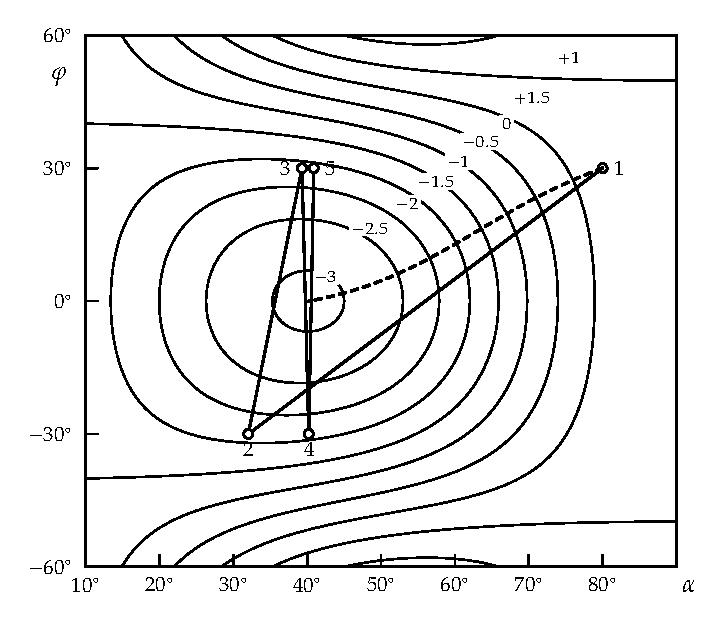
\includegraphics[width=0.75\textwidth]{pictures/5_3}
\par\end{centering}
\caption{\label{fig:5_3}通过迭代对角化（实线）与梯度法（虚线）求解HF方程的数值比较。}
\end{figure}


\section{Hartree-Fock方法与对称性\label{sec:Hartree-Fock=0065B9=006CD5=004E0E=005BF9=0079F0=006027}}

HF方程是非线性的，这意味这自洽势$\Gamma$不仅依赖于Hamilton量，也依赖于解（由密度矩阵$\rho$表示）。因此，这个势和Hamilton量不具有相同的对称性。我们由此可以说这个解的对称性破缺了。平移不变性的破缺我们已经遇到过，不过除此之外还有转动对称性和粒子数对称性（见\ref{chap:=005BF9=005173=008054=004E0E=008D85=006D41=006838}和\ref{chap:=0063A8=005E7F=007684=005355=007C92=005B50=006A21=00578B=00FF08HFB=007406=008BBA=00FF09}）通常人们会把从对称性保持到破缺的过程称为相变。这种对称性破缺的最大有点就是允许我们在简单的单粒子图像下去近似地考虑多体关联。更为细致的讨论将会在\ref{chap:=0063A8=005E7F=007684=005355=007C92=005B50=006A21=00578B=00FF08HFB=007406=008BBA=00FF09}，\ref{chap:=005BF9=0079F0=006027=007684=006062=00590D}和\ref{chap:=0076F4=0079EF=006CE2=0051FD=006570=0076F8=005173=007684=005B9A=007406}中给出，我们这里仅仅做如下论述：假设我们由一个Slater行列式$|\Phi\rangle$，它由形变的单粒子基$\{a^{\dagger}_{k}\}$组成。我们可以通过线性变换用球形基把它表示出来：
\[
a^{\dagger}_{k}=\sum_{q}D_{qk}c^{\dagger}_{q}
\]

我们因此得到了一系列球形基下占据数不同的Slater行列式之和：
\[
a^{\dagger}_{i_{1}}\dots a^{\dagger}_{i_{N}}|-\rangle=\sum_{q_{1}\dots q_{N}}d^{i_{1}\dots i_{N}}_{q_{1}\dots q_{N}}c^{\dagger}_{q_{1}}\dots c^{\dagger}_{q_{N}}|-\rangle
\]

这里系数$d^{i_{1}\dots i_{N}}_{q_{1}\dots q_{N}}$是一系列矩阵$D_{qk}$的乘积。当然，这种符号实际上对应着更一般的拟设，它包含了精确解，当然它绝对不是能用HF波函数描述的
\begin{comment}
原文经典不说人话，我这里翻译的已经尽量是人话了。这里实际上想说这个符号是个张量的符号，这种张量一般不能写成矩阵的张量积。如果这里真的是个一般的张量的话，这种形式的波函数应该可以张成整个空间，所以一定包含精确解。但是这个精确解一般来说写不成HF波函数的形式。
\end{comment}
。不论如何，我们可以看出一组基下的Slater行列式在另一组基下可能十分复杂，是一系列Slater行列式的叠加态。

当然，精确的波函数应当由Hamilton量的对称性，对称性的破缺只是因为我们想尽可能的维持独立粒子的图像。尽管如此，我们之后会尝试恢复破缺掉的对称性。我们将在\ref{chap:=005BF9=0079F0=006027=007684=006062=00590D}讨论这一点。然而，HF理论确实保留了特定的对称性，也就是所谓的自洽对称性。它们依赖于初始的密度$\rho^{(0)}$，以及HF场$\Gamma$：
\begin{equation}
S\Gamma[\rho]S^{\dagger}=\Gamma[S\rho S^{\dagger}]\label{eq:self-consistence sysmmetry}
\end{equation}

\begin{booknote*}
定理：如果 $S$ 是一个对称算符（酉算符或反酉算符），且与Hamilton量对易，那么有 $Sh[\rho]S^{-1}=h[S\rho S^{-1}]$。

证明（酉算符情景）：我们假设算符 $S$ 作用到产生算符上有：

\[
Sa^{\dagger}_{i}S^{-1}=\sum_{ii^{\prime}}S_{ii^{\prime}}a^{\dagger}_{i^{\prime}}
\]

则其作用到湮灭算符上有：

\[
Sa_{i}S^{-1}=\sum_{ii^{\prime}}S^{*}_{ii^{\prime}}a_{i^{\prime}}
\]

我们记其作用到态 $|i\rangle$ 后使其变为 $|\bar{i}\rangle$，根据上面的假设，我们可以把它用原来的基展开，得到：

\[
S|i\rangle=|\bar{i}\rangle=\sum_{i^{\prime}}S_{ii^{\prime}}|i^{\prime}\rangle
\]

单粒子密度矩阵为 $\rho_{ij}=\mathop{\text{Tr}}(\rho a^{\dagger}_{j}a_{i})$，对其做对称操作后记为$\bar{\rho}_{ij}$，即得到：

\[
\begin{aligned}\bar{\rho}_{ij} & =\mathop{\text{Tr}}(S\rho a^{\dagger}_{j}a_{i}S^{-1})\\
 & =\mathop{\text{Tr}}(\rho Sa^{\dagger}_{j}S^{-1}Sa_{i}S^{-1})\\
 & =\sum_{i^{\prime}j^{\prime}}S^{*}_{ii^{\prime}}S_{jj^{\prime}}\mathop{\text{Tr}}(\rho a^{\dagger}_{j^{\prime}}a_{i^{\prime}})\\
 & =\sum_{i^{\prime}j^{\prime}}S^{*}_{ii^{\prime}}S_{jj^{\prime}}\rho_{i^{\prime}j^{\prime}}
\end{aligned}
\]

对 HF Hamilton量做对称操作，即得到：

\[
\begin{aligned}\langle\bar{k}|h|\bar{l}\rangle & =\langle\bar{k}|t|\bar{l}\rangle+\sum_{ij}\langle\bar{k}i|V|\bar{l}j\rangle\rho_{ij}\\
 & =\langle\bar{k}|t|\bar{l}\rangle+\sum_{ij}\sum_{i^{\prime}j^{\prime}}S_{i^{\prime}i}S^{*}_{j^{\prime}j}\langle\bar{k}\bar{i^{\prime}}|V|\bar{l}\bar{j^{\prime}}\rangle\rho_{ij}\\
 & =\langle\bar{k}|t|\bar{l}\rangle+\sum_{ij}\langle\bar{k}\bar{i}|V|\bar{l}\bar{j}\rangle\bar{\rho}_{ij}\\
 & =\langle k|t|l\rangle+\sum_{ij}\langle ki|V|lj\rangle\bar{\rho}_{ij}
\end{aligned}
\]

证毕。这里要用到$\rho_{ij}=\rho_{ji}$。

推论：如果$S$保持单粒子密度矩阵不变，那么其与HFHamilton量$h$对易。（$S$保持单粒子密度矩阵不变等价于$\sum_{i^{\prime}j^{\prime}}S^{*}_{ii^{\prime}}S_{jj^{\prime}}\rho_{i^{\prime}j^{\prime}}=\rho_{ij}$，在零温下这等价于保持占据态不变。）

证明：

由于$S\rho S^{-1}=\rho$，由此$Sh[\rho]S^{-1}=h[S\rho S^{-1}]=h[\rho]$。即$S$与$h$对易。

推论：如果$\rho$在迭代中初始保持了一定的对称性，那么其之后一直保持这种对称性。

满足这一性质的有：偶偶核中的时间反演算符，宇称算符，忽略库伦相互作用时$N=Z$核中的同位旋交换算符，闭壳核（球对称）中的角动量算符，轴对称核中的对称轴方向角动量算符，忽略自旋轨道耦合项时的自旋算符。
\end{booknote*}
这意味着如果初始密度$\rho^{(0)}$具有特定的Hamilton量具有的对称性$S$，那么第一步得到的自洽场$h[\rho^{(0)}]$也如此。而下一步的密度$\rho^{(1)}$是通过对$h[\rho^{(0)}]$
\begin{comment}
原文$h[\rho^{(1)}]$
\end{comment}
对角化得到的，由此它必须具有相同的对称性。由此，在每一步迭代中，对称性$S$都被保留了。

自洽对称性的存在对实际的计算有以下影响\cite{Ri68}：
\begin{enumerate}
\item 如果我们期待最终的解具有特定的对称性，我们可以让初始密度$\rho^{(0)}$具有这个对称性，因此计算只在具有该对称性的基上进行，计算量就减小了。
\item 如果我们从特定对称性出发，我们将只能得到具有对称性的解，即最小能量是在具有这种对称性的波函数上变分得到的。例如，假如极小值是一个形变Slater行列式，但我们从一个球对称的密度矩阵出发，我们将永远也得不到这个解，尽管微小的数值误差可能让最终的解有微小的形变。
\item 如果我们有一个对称性$S$被破缺掉的解：
\[
S\rho S^{\dagger}=\rho_{1}\neq\rho
\]
那么从\ref{eq:self-consistence sysmmetry}可以得到变换后的密度对应的HFHamilton量$h[\rho_{1}]$：
\[
h[\rho_{1}]=S^{\dagger}h[\rho]S
\]
这意味着$\rho_{1}$也是HF方程的解：
\[
[h[\rho_{1}],\rho_{1}]=0
\]
在连续对称性的情况下，例如平移对称性和转动对称性，对一个对称性破缺的解，我们可以找到无数个简并的解。
\end{enumerate}
在下一节，我们将会看到密度依赖的两体相互作用在HF计算中的作用。在这种情况下，核力不一定再具有和裸核力一样的对称性。尽管如此，HF解在对称变换下的通常的性质依然会成立。只要我们要求相互作用满足一个非常宽松的性质：
\[
\hat{S}V[\rho]\hat{S}^{-1}=V[S\rho S^{-1}]
\]

以转动为例，这意味着一个转动过的系统中两体相互作用和用转动过的密度计算出来的相互作用相同。Skyrme力就满足这个条件。

\section{Hartree-Fock方法与密度依赖相互作用\label{sec:Hartree-Fock=0065B9=006CD5=004E0E=005BC6=005EA6=004F9D=008D56=0076F8=004E92=004F5C=007528}}

\subsection{有效相互作用方法\label{subsec:=006709=006548=0076F8=004E92=004F5C=007528=0065B9=006CD5}}

\subsubsection{Brückner-Hartree-Fock\label{subsubsec:Brueckner-Hartree-Fock}}

直接应用前面各节所述的Hartree-Fock方法的一个主要障碍在于，大多数裸核子-核子力都具有无穷大或者至少是非常强烈的排斥芯（参见第4章）。容易验证，对于硬芯势，进入Hartree-Fock势式(5.34)的两体矩阵元全都会发散到无穷大。解决这一困难的途径，是用第4.3.1节中讨论的Brückner$G$矩阵替换式(5.34)中的裸相互作用。事实上，这不仅因为解决了硬芯问题而带来便利，而且还可以证明，它是对整个多体问题中某些特定高阶项的自洽求和重整化（resummation）。由于我们此处手头尚未建立起完备的多体理论数学工具，我们将这一证明留到附录F.4中。

仿照式(5.38)，Brückner-Hartree-Fock（BHF）方程可写为（亦可参阅H. S. Köhler \cite{Ko75}以及W.
Wild \cite{Wi77}关于该主题的综述）：

\begin{equation}
\sum_{l'}\left\{ t_{ll'}+\sum^{A}_{i=1}\sum_{pp'}G^{\epsilon_{k}+\epsilon_{i}}_{lp',l'p}D_{pi}D^{*}_{p'i}\right\} D_{l'k}=\epsilon_{k}D_{lk}\label{eq:bhf_equation}
\end{equation}

这里$G$是由式(4.39)定义的Brückner$G$矩阵，是用某一特定单粒子势的基矢展开表示的。在作为式(5.72)之解的基矢中，相应的基态能量由下式给出：

\begin{align}
E^{\mathrm{BHF}}_{0} & =\sum^{A}_{i=1}t_{ii}+\frac{1}{2}\sum^{A}_{i,j=1}G^{\epsilon_{i}+\epsilon_{j}}_{ij,ij}\label{eq:bhf_e0_t}\\
 & =\sum^{A}_{i=1}\epsilon_{i}-\frac{1}{2}\sum^{A}_{i,j=1}G^{\epsilon_{i}+\epsilon_{j}}_{ij,ij}\label{eq:bhf_e0_eps}
\end{align}

对于基态能量而言，我们似乎只需要\ref{eq:bhf_equation}的空穴解。然而，\ref{eq:bhf_equation}的粒子解通过中间粒子能量$\epsilon_{n},\epsilon_{m}$进入到Bethe-Goldstone方程(4.39)中。因此，Brückner-Hartree-Fock解包含了一个复杂的双重自洽迭代过程。例如，可以通过如下迭代循环来求解：(i)
在初选的一组适宜基矢（例如简谐振子基）中通过式(4.39)计算$G$矩阵；(ii) 在该基矢下将\ref{eq:bhf_equation}对角化一次，得到一组新的基矢；(iii)
在这组新基矢下计算新的$G$矩阵；如此重复，直至达到自洽收敛。

然而，在这一迭代循环中，关于\ref{eq:bhf_equation}中$G$矩阵的能量依赖性会出现某种细微的歧义。由于我们事先并不知道最终的解，因此必须将$G^{\epsilon_{k}+\epsilon_{i}}_{lp',l'p}$的能量依赖性纳入迭代循环中。这样，在迭代的每一步中，我们必须取$\epsilon_{k}$为实际写出\ref{eq:bhf_equation}所在基矢对应的能量，即可以取$\epsilon_{k}$等于$\epsilon_{l}$或$\epsilon_{l'}$。对于$\epsilon_{i}$则不存在歧义，因为在迭代过程中$D_{pi}$被取为对角阵。对于BHF势能矩阵{[}参见式(5.34){]}，通常的约定取法是（参见例如\cite{Ba69a}；当然，最终的结果并不依赖于任何具体的约定）：

\begin{equation}
\Gamma^{\mathrm{BHF}}_{kk'}=\begin{cases}
\frac{1}{2}\sum^{A}_{i=1}\left(G^{\epsilon_{k}+\epsilon_{i}}_{ki,k'i}+G^{\epsilon_{k'}+\epsilon_{i}}_{ki,k'i}\right) & \text{当 }k,k'\leqslant\epsilon_{F},\\
\sum^{A}_{i=1}G^{\epsilon_{k}+\epsilon_{i}}_{ki,k'i} & \text{当 }k\leqslant\epsilon_{F},\,k'>\epsilon_{F},\\
\sum^{A}_{i=1}G^{\epsilon_{k'}+\epsilon_{i}}_{ki,k'i} & \text{当 }k'\leqslant\epsilon_{F},\,k>\epsilon_{F}.
\end{cases}\label{eq:bhf_gamma}
\end{equation}

$\Gamma^{\mathrm{BHF}}$的粒子-粒子矩阵元是一个略有争议的问题。对于给定的$G$矩阵，$\Gamma^{\mathrm{BHF}}$的粒子-粒子矩阵元并不直接影响\ref{eq:bhf_equation}的空穴解；然而，它们确实会影响粒子解，并进而通过双重自洽循环中的式(4.39)，间接地影响空穴解。我们可以证明（参见\cite{Ba69a,Ne70}中的讨论）：如果令$\Gamma^{\mathrm{BHF}}$的粒子-粒子矩阵元等于零，即

\begin{equation}
\Gamma^{\mathrm{BHF}}_{kk'}=0,\quad\text{当 }k,k'>\epsilon_{F},\label{eq:bhf_gamma_pp}
\end{equation}

那么原本在我们最初的\ref{eq:bhf_equation}和式(4.39)表述中所没有的三体关联就得到了有效的求和贡献。

\ref{eq:bhf_equation}不仅因为两体算符更加复杂而有别于通常的HF方程(5.38)，而且还因为$\Gamma^{\mathrm{BHF}}$现在依赖于我们想要计算的本征能量。因此，这是一个非线性问题，其中对应不同能量的解通常不再严格正交（但在球对称情况下，具有不同角动量的解依然是正交的）。然而，对于迭代求解而言，这并没有特别的妨碍\footnote{不过，人们仍然需要确保$\Gamma^{\mathrm{BHF}}$的能量依赖性不要过强，否则独立粒子图像可能不再成立。}。

正如我们在第4.3.1节所讨论的，$G$矩阵对核介质中的两粒子散射过程进行了求和。可以证明，\ref{eq:bhf_e0_eps}包含了此类过程对基态能量的全部贡献\cite{Ma67b}。在\ref{tab:bhf_results_reid}中，我们给出了以Reid软芯势(4.35)作为裸核力时，对$^{16}\mathrm{O}$、$^{40}\mathrm{Ca}$和$^{208}\mathrm{Pb}$进行Brückner-Hartree-Fock计算得到的方均根半径和单核子结合能。

\begin{table}[H]
\begin{centering}
\caption{\label{tab:bhf_results_reid}使用Reid软芯势的BHF计算结果与实验值的比较（来自\cite{DMS73}）}
\par\end{centering}
\centering{}%
\begin{tabular}{|c|c|c|c|}
\hline 
核素 & 物理量 & BHF & 实验值\tabularnewline
\hline 
\hline 
$^{16}\mathrm{O}$ & $-E_{0}/A\ (\mathrm{MeV})$ & 3.91 & 7.98\tabularnewline
 & $\mathrm{rms}\ (\mathrm{fm})$ & 2.50 & 2.73\tabularnewline
\hline 
$^{40}\mathrm{Ca}$ & $-E_{0}/A$ & 3.88 & 8.55\tabularnewline
 & $\mathrm{rms}$ & 3.04 & 3.48\tabularnewline
\hline 
$^{208}\mathrm{Pb}$ & $-E_{0}/A$ & 2.52 & 7.87\tabularnewline
 & $\mathrm{rms}$ & 4.51 & 5.50\tabularnewline
\hline 
\end{tabular}
\end{table}

\ref{tab:bhf_results_reid}中的结果是令人失望的。计算得到的结合能甚至还不到实验值的一半，而方均根半径也有约10\%–20\%的偏差。不过，结合能结果不佳并不十分令人意外，因为它是动能和势能这两个非常大的数值之间相抵消的差值。

然而，面对这一令人不满意的结果，人们必须考虑计入更复杂的过程\footnote{在此背景下，亦可参见超网链（hypernetted chain）形式体系\cite{PB73,FR75,FR76a,LS77,Ri79}。}。在多体阶层结构中，下一层便是三粒子散射项，其重要性应当依赖于系统的密度。正如我们在第4.3节中所看到的，表征两粒子关联力程的愈合距离（healing
distance）明显小于核子间的平均距离。因此，三个粒子同时处于愈合距离范围内的概率应当相当小。然而，这只是一个定性的论证\cite[p. 161]{Be71}。事实上，Kümmel及其合作者已经能够以完全自洽的方式将三体关联纳入基态能量的计算中（参见例如\cite{KLZ75,KLZ78}以及其中引用的文献）。他们还给出了强有力的论据，表明四体关联应当可以忽略。他们的结果非常引人注目，其与实验的符合程度得到了改善，尽管并不是非常剧烈。对于不同的核子-核子势，计算结果在$-E_{0}/A$与方均根半径平面上大致分布在一条光滑曲线上，如\ref{fig:bhf_coester_line}所示。这条曲线被称为Coester线（Coester
line）。Reid软芯势的结果大约位于该曲线最接近实验值的点上。鉴于文献\cite{KLZ75}中关于结果已经收敛的论断，剩余的差异必须归因于相对论效应或介子自由度。

\begin{figure}[H]
\begin{centering}
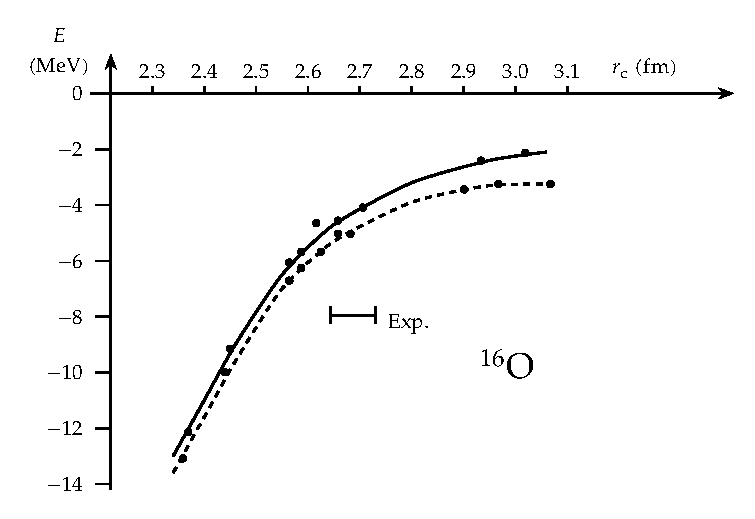
\includegraphics[width=0.75\linewidth]{pictures/5_4}
\par\end{centering}
\centering{}\caption{\label{fig:bhf_coester_line}不同核子-核子势的BHF计算结果（实线上的圆点）与包含三体关联的计算结果（虚线）以及实验值的比较（引自\cite{Wi77}）}
\end{figure}


\subsubsection{局域密度近似和变分原理\label{subsubsec:=005C40=0057DF=005BC6=005EA6=008FD1=004F3C=00548C=0053D8=005206=00539F=007406}}

在第4.3节中，我们看到硬芯势对两核子波函数的影响主要发生在其相对距离从0到约$1\,\mathrm{fm}$的范围内，也就是说，与大约$10\,\mathrm{fm}$的原子核半径相比，仅仅作用在非常短的距离上。这意味着Brückner$G$矩阵仅在相同的$r$值范围内才显著不同于裸相互作用$v(r)$。然而，一般而言，两核子相对坐标$r=|\boldsymbol{r}_{1}-\boldsymbol{r}_{2}|$约$1\,\mathrm{fm}$的变动，意味着质心坐标也有相近尺度的变化。核密度$\rho(\boldsymbol{R})=\rho(\frac{1}{2}(\boldsymbol{r}_{1}+\boldsymbol{r}_{2}))$在这样大小的$\boldsymbol{R}$范围内并不会发生很大改变（至少在核内部是如此）。因此，在每个$\rho(\boldsymbol{R})$值处计算核$G$矩阵时，假设原子核在$\boldsymbol{R}$附近的局域表现得就像是一块密度为$\rho(\boldsymbol{R})$的核物质\footnote{关于核物质理论，参见综述文献\cite{Be71,Sp72,JLM76}。}，这似乎是一个非常合理的假设。事实上，这种论证思路与Thomas-Fermi近似（参见第13章）非常接近。更明确地说，这意味着在利用\ref{eq:bhf_gamma_pp}写出的Bethe-Goldstone方程(4.39)中：

\begin{equation}
G^{W}=\bar{v}+\bar{v}\frac{Q_{F}}{W-Q_{F}\Gamma Q_{F}}G^{W}\label{eq:bg_gw}
\end{equation}

我们将投影算符$Q_{F}$替换为它在密度为$\rho(\boldsymbol{R})$的核物质中的表达式$Q^{\mathrm{NM}}_{F}$。由于$Q_{F}$式(4.41)可以由非局域单粒子密度$\rho(\boldsymbol{r},\boldsymbol{r}')=\sum^{A}_{i=1}\varphi_{i}(\boldsymbol{r})\varphi^{*}_{i}(\boldsymbol{r}')$表示为：

\begin{equation}
\langle\boldsymbol{r}_{1}\boldsymbol{r}_{2}|Q_{F}|\boldsymbol{r}'_{1}\boldsymbol{r}'_{2}\rangle=[\delta(\boldsymbol{r}_{1}-\boldsymbol{r}'_{1})-\rho(\boldsymbol{r}_{1},\boldsymbol{r}'_{1})][\delta(\boldsymbol{r}_{2}-\boldsymbol{r}'_{2})-\rho(\boldsymbol{r}_{2},\boldsymbol{r}'_{2})]\label{eq:qf_matrix_elem}
\end{equation}

这意味着在\ref{eq:qf_matrix_elem}中，$\rho$必须替换为其核物质中的取值{[}参见式(13.20){]}：

\begin{equation}
\rho^{\mathrm{NM}}(\boldsymbol{r},\boldsymbol{r}')=\frac{3}{k_{F}(\boldsymbol{R})s}j_{1}(k_{F}(\boldsymbol{R})s)\rho(\boldsymbol{R})\label{eq:rho_nm}
\end{equation}

其中$\boldsymbol{s}=\boldsymbol{r}-\boldsymbol{r}'$，$\boldsymbol{R}=\frac{1}{2}(\boldsymbol{r}+\boldsymbol{r}')$，$j_{1}$是球Bessel函数。\ref{eq:rho_nm}对$\boldsymbol{R}$的依赖性来源于我们仅在$\boldsymbol{R}$附近将原子核局域地当作核物质处理。$k_{F}$与$\rho$之间的关系一如既往地由下式给出{[}参见式(5.91)、式(13.22)和式(13.23){]}：

\begin{equation}
\rho(\boldsymbol{R})=\frac{2}{3\pi^{2}}k^{3}_{F}(\boldsymbol{R})\label{eq:rho_kf_rel}
\end{equation}

与有限核精确密度矩阵的数值比较表明\cite{Ne75}，在原子核内部，$\rho$的非局域行为能被\ref{eq:rho_nm}极其优良地近似，并且在整个核表面区域也得到了合理的再现。因此我们可以得出结论：此处所描述的对$G$矩阵的局域密度近似是相当成功的。

原则上，以此种方式计算的$G$矩阵依赖于三个变量：$\boldsymbol{r}=\boldsymbol{r}_{1}-\boldsymbol{r}_{2}$、$\boldsymbol{r}'=\boldsymbol{r}'_{1}-\boldsymbol{r}'_{2}$以及$\boldsymbol{R}=\frac{1}{2}(\boldsymbol{r}_{1}+\boldsymbol{r}_{2}-\boldsymbol{r}'_{1}-\boldsymbol{r}'_{2})$，即$G=G_{\boldsymbol{r},\boldsymbol{r}';\boldsymbol{R}}$。然而事实表明，$G$对总动量$\boldsymbol{P}$（与$\boldsymbol{R}$共轭的变量）的依赖性很弱，通常我们将其置为其平均值\cite{BGW58}：

\[
G_{\boldsymbol{r},\boldsymbol{r}';\boldsymbol{P}}\simeq G_{\boldsymbol{r},\boldsymbol{r}';\boldsymbol{P}_{\mathrm{av}}}
\]

Negele \cite{Ne70}进一步简化了$G$的表达式。他将式(5.73)的$G$矩阵中出现的起始能量$W=\epsilon_{i}+\epsilon_{j}$替换为一个平均值，该平均值取为核物质中平均空穴能量的两倍。通过这种方式，我们消除了式(5.72)中单粒子势对态的依赖性，相应的本征函数系构成了一组完备的正交归一基。下一步则是用一个有效局域算符$v^{\mathrm{eff}}(\boldsymbol{r})$来表示$G_{\boldsymbol{r},\boldsymbol{r}'}$（我们略去具体实现的细节，读者可参阅文献\cite{Ne70}\footnote{关于“局域”密度近似的其他应用，参见\cite{Ko65,NV70,CS72,NR72}。}）。此外，该有效相互作用经过唯象的重整化，以给出正确的核物质体积能项{[}参见Bethe-Weizsäcker公式(1.4){]}。从这个意义上说，Negele的“密度依赖HF”（DDHF）方法仍然是一种半唯象的方案。

Negele理论中还有一个至关重要的要素我们此前尚未提及：在\ref{tab:bhf_results_reid}中，我们看到纯粹的BHF计算并不能给出令人满意的结果；因此，必须寻求更好的方法。事实证明，将基态能量(5.73)中的$G$替换为局域密度近似，并像纯HF情况那样{[}式(5.29){]}对单粒子波函数进行能量变分，这一极具直观吸引力的构想带来了极好的计算结果。在这种情况下，Hartree-Fock
Hamilton量变为{[}参见式(5.32){]}：

\begin{equation}
h^{\mathrm{HF}}_{kk'}=\frac{\delta E[\rho]}{\delta\rho_{k'k}}=t_{kk'}+\sum_{qq'}\bar{v}^{\mathrm{eff}}_{kq'k'q}\rho_{qq'}+\left\langle \Phi\left|\frac{\delta v^{\mathrm{eff}}}{\delta\rho_{k'k}}\right|\Phi\right\rangle \label{eq:ddhf_h_var}
\end{equation}

其中$|\Phi\rangle$是与密度$\rho$对应的Slater行列式。对于密度无关的力，式(5.81)直接还原为通常的HF
Hamilton量。然而对于密度依赖的力，我们多出了一个附加项$\delta v^{\mathrm{eff}}/\delta\rho$，通常称之为重排势（rearrangement
potential）或饱和势（saturation potential）。它源自$v^{\mathrm{eff}}(\rho)$中的密度依赖性，并在实际数值计算中起着极其重要的作用。但必须强调的是，刚才所描述的变分方法并不等价于通过试探波函数变分来极小化原始多体Hamilton量(5.25)的期望值。这意味着，至少在原则上，由\ref{eq:ddhf_h_var}计算出的基态能量有可能低于真实的精确能量。该方法的合理性首先建立在其巨大的成功之上；在理论上，我们可以说附加项$\delta v^{\mathrm{eff}}/\delta\rho$在某种程度上计入了三体散射项\cite{Ne75}（在壳模型空间中，$\delta v^{\mathrm{eff}}/\delta\rho$具有六个指标）。在\ref{tab:ddhf_results}中，我们展示了使用DDHF方法相比于BHF所取得的显著改善\cite{Ne70,NV75}。

\begin{table}[H]
\begin{centering}
\caption{\label{tab:ddhf_results}密度依赖Hartree-Fock方法（DDHF）计算的结合能（以MeV为单位）与方均根半径（以fm为单位）}
\par\end{centering}
\centering{}%
\begin{tabular}{|c|c|c|c|c|}
\hline 
核素 & 物理量 & BHF & DDHF & 实验值\tabularnewline
\hline 
\hline 
$^{16}\mathrm{O}$ & $-E_{0}/A$ & 3.91 & 7.59 & 7.98\tabularnewline
 & $\mathrm{rms}$ & 2.50 & 2.75 & 2.73\tabularnewline
\hline 
$^{40}\mathrm{Ca}$ & $-E_{0}/A$ & 3.88 & 7.99 & 8.55\tabularnewline
 & $\mathrm{rms}$ & 3.04 & 3.46 & 3.48\tabularnewline
\hline 
$^{208}\mathrm{Pb}$ & $-E_{0}/A$ & 2.52 & 7.83 & 7.87\tabularnewline
 & $\mathrm{rms}$ & 4.51 & 5.49 & 5.50\tabularnewline
\hline 
\end{tabular}
\end{table}

求解DDHF方程是一项非常复杂的任务，因为交换项(5.43)意味着必须求解一个积分微分方程。然而，核力具有相当短的力程这一事实可以被用来简化问题，从而使得非局域交换项可以围绕其局域值按非局域程度进行展开。这种方法极其自然地为采用唯象Skyrme力的非常成功的HF方案提供了理论辩护，我们将在接下来研究这一方案\cite{Ne75}。

\subsection{Skyrme力的Hartree-Fock计算\label{subsec:Skyrme=00529B=007684Hartree-Fock=008BA1=007B97}}

\subsubsection{一般评述\label{subsubsec:=004E00=00822C=008BC4=008FF0}}

已经有许多不同的核力用于Hartree-Fock方法的计算。对这些核力给出一个综述超出了本书的范围（对于最近的综述，见\cite{QF78}）。他们中的许多——尤其是没有使用密度依赖项的核力——不能同时描述好结合能，半径，以及轻核和重核的正确的单粒子能谱（例如，\cite{Vo65,MB65,BB67,NDK68,PS68,SFW69,SP70}）。

Skyrme力作为一个唯象核力，很好的复现了整个元素周期表的结合能和半径\footnote{有一大批相似的唯象的密度依赖零程\cite{Mo70,LV71,La72,EM72,BJS75,Ko76,LB76,TK76,KKS77,SM78}或者有限程\cite{Kr70,ZR71,RPS72,LMV73,Go75b,RBP77}核力在HF计算中表现出了和Skyrme力相似的性质。}。同由局域密度近似得到的Negele力一样，Skyrme力是密度依赖的，不能在变分原理中简单的直接利用。形式上讲，这一困难可以通过把Skyrme力考虑成三体力来克服。

\subsubsection{利用Skyrme力计算能量\label{subsubsec:=005229=007528Skyrme=00529B=008BA1=007B97=0080FD=0091CF}}

我们从式(4.104)给出的Skyrme力出发，计算相应的Hamilton量在由单粒子波函数$\varphi_{i}(\boldsymbol{r},\sigma,q)$构成的Slater行列式$|\Phi\rangle$下的期望值。这里$\sigma=\pm\frac{1}{2}$是自旋量子数，$q=\pm\frac{1}{2}$是电荷量子数（质子或中子）。我们将波函数写为二分量旋量：

\begin{equation}
\varphi_{i}(\boldsymbol{r},\sigma,q)=\varphi_{i}(\boldsymbol{r},q)\chi_{\sigma_{i}}(\sigma)=\left(\begin{array}{c}
\varphi_{i}(\boldsymbol{r},q,\frac{1}{2})\\
\varphi_{i}(\boldsymbol{r},q,-\frac{1}{2})
\end{array}\right)\label{eq:skyrme_spinor}
\end{equation}

单粒子密度矩阵在坐标表象中具有如下形式{[}参见式(C.16){]}：

\begin{equation}
\rho(\boldsymbol{r}\sigma q,\boldsymbol{r}'\sigma'q')=\langle\Phi|a^{\dagger}_{\boldsymbol{r}'\sigma'q'}a_{\boldsymbol{r}\sigma q}|\Phi\rangle=\delta_{qq'}\rho_{q}(\boldsymbol{r}\sigma,\boldsymbol{r}'\sigma')\label{eq:density_matrix_coord}
\end{equation}

其中质子和中子的密度矩阵互不混合。总密度矩阵由下式给出：

\begin{equation}
\rho(\boldsymbol{r}\sigma,\boldsymbol{r}'\sigma')=\rho_{p}(\boldsymbol{r}\sigma,\boldsymbol{r}'\sigma')+\rho_{n}(\boldsymbol{r}\sigma,\boldsymbol{r}'\sigma')=\sum^{A}_{i=1}\varphi_{i}(\boldsymbol{r},\sigma,q_{i})\varphi^{*}_{i}(\boldsymbol{r}',\sigma',q_{i})\label{eq:total_density_matrix}
\end{equation}

为了计算结合能，我们需要如下局域密度量\cite{VB72}：

(i) 核子密度：

\begin{align}
\rho_{q}(\boldsymbol{r}) & =\sum_{\sigma}\rho_{q}(\boldsymbol{r}\sigma,\boldsymbol{r}\sigma)=\sum^{A}_{i=1}\delta_{q_{i}q}\sum_{\sigma}|\varphi_{i}(\boldsymbol{r},\sigma,q)|^{2}\label{eq:rho_q_def}\\
\rho(\boldsymbol{r}) & =\rho_{p}(\boldsymbol{r})+\rho_{n}(\boldsymbol{r})\label{eq:rho_tot_def}
\end{align}

(ii) 动能密度：

\begin{align}
\tau_{q}(\boldsymbol{r}) & =\sum_{\sigma}\left[\boldsymbol{\nabla}\cdot\boldsymbol{\nabla}'\rho_{q}(\boldsymbol{r}\sigma,\boldsymbol{r}'\sigma)\right]_{\boldsymbol{r}=\boldsymbol{r}'}=\sum^{A}_{i=1}\delta_{q_{i}q}\sum_{\sigma}|\boldsymbol{\nabla}\varphi_{i}(\boldsymbol{r},\sigma,q)|^{2}\label{eq:tau_q_def}\\
\tau(\boldsymbol{r}) & =\tau_{p}(\boldsymbol{r})+\tau_{n}(\boldsymbol{r})\label{eq:tau_tot_def}
\end{align}

(iii) 自旋-轨道（流）密度矢量：

\begin{align}
\boldsymbol{J}_{q}(\boldsymbol{r}) & =(-\mathrm{i})\sum_{\sigma\sigma'}\left[\boldsymbol{\nabla}\rho_{q}(\boldsymbol{r}\sigma,\boldsymbol{r}'\sigma')\times\langle\sigma|\boldsymbol{\sigma}|\sigma'\rangle\right]_{\boldsymbol{r}=\boldsymbol{r}'}\nonumber \\
 & =(-\mathrm{i})\sum^{A}_{i=1}\delta_{q_{i}q}\sum_{\sigma\sigma'}\varphi^{*}_{i}(\boldsymbol{r},\sigma',q)\left[\boldsymbol{\nabla}\varphi_{i}(\boldsymbol{r},\sigma,q)\times\langle\sigma'|\boldsymbol{\sigma}|\sigma\rangle\right]\label{eq:J_q_def}\\
\boldsymbol{J}(\boldsymbol{r}) & =\boldsymbol{J}_{p}(\boldsymbol{r})+\boldsymbol{J}_{n}(\boldsymbol{r})\label{eq:J_tot_def}
\end{align}

利用这些密度量，总能量期望值可以表示为一个能量密度的空间积分：

\begin{equation}
E=\langle\Phi|H|\Phi\rangle=\int\mathcal{H}(\boldsymbol{r})\,\mathrm{d}^{3}r\label{eq:skyrme_E_integral}
\end{equation}

由于Skyrme力的零程特性以及只保留到动量二阶项的动量依赖性，Hamilton能量密度泛函$\mathcal{H}(\boldsymbol{r})$完全是局域的。它由动能项、Skyrme相互作用能密度以及Coulomb能密度三部分构成：

\begin{equation}
\mathcal{H}(\boldsymbol{r})=\frac{\hbar^{2}}{2m}\tau(\boldsymbol{r})+\mathcal{H}_{\mathrm{Skyrme}}(\boldsymbol{r})+\mathcal{H}_{\mathrm{Coul}}(\boldsymbol{r})\label{eq:skyrme_H_density}
\end{equation}

对于时间反演不变的球对称或轴对称偶偶核系统，Skyrme相互作用能密度具有如下优美而紧凑的形式：

\begin{align}
\mathcal{H}_{\mathrm{Skyrme}}(\boldsymbol{r}) & =\frac{1}{2}t_{0}\left[\left(1+\frac{1}{2}x_{0}\right)\rho^{2}-\left(x_{0}+\frac{1}{2}\right)(\rho^{2}_{p}+\rho^{2}_{n})\right]\nonumber \\
 & \quad+\frac{1}{4}\left(t_{1}+t_{2}\right)\rho\tau+\frac{1}{8}\left(t_{2}-t_{1}\right)(\rho_{p}\tau_{p}+\rho_{n}\tau_{n})\nonumber \\
 & \quad+\frac{1}{16}\left(t_{2}-3t_{1}\right)\rho\nabla^{2}\rho+\frac{1}{32}\left(3t_{1}+t_{2}\right)(\rho_{p}\nabla^{2}\rho_{p}+\rho_{n}\nabla^{2}\rho_{n})\nonumber \\
 & \quad+\frac{1}{4}t_{3}\rho_{p}\rho_{n}\rho-\frac{1}{2}W_{0}\left[\rho\boldsymbol{\nabla}\cdot\boldsymbol{J}+\rho_{p}\boldsymbol{\nabla}\cdot\boldsymbol{J}_{p}+\rho_{n}\boldsymbol{\nabla}\cdot\boldsymbol{J}_{n}\right]\nonumber \\
 & \quad+\frac{1}{16}\left(t_{1}-t_{2}\right)\left[\boldsymbol{J}^{2}_{p}+\boldsymbol{J}^{2}_{n}\right]-\frac{1}{32}\left(t_{1}+t_{2}\right)\boldsymbol{J}^{2}\label{eq:H_skyrme_full}
\end{align}

在具有对称核物质密度（$\rho_{n}=\rho_{p}=\frac{1}{2}\rho$）的情况下，自旋-轨道密度相互抵消，\ref{eq:H_skyrme_full}显著简化为仅依赖于标量密度的形式：

\begin{align}
\mathcal{H}_{\mathrm{Skyrme}}(\boldsymbol{r}) & =\frac{3}{8}t_{0}\rho^{2}+\frac{1}{16}t_{3}\rho^{3}+\frac{1}{16}\left(3t_{1}+5t_{2}\right)\rho\tau\nonumber \\
 & \quad+\frac{1}{64}\left(9t_{1}-5t_{2}\right)(\boldsymbol{\nabla}\rho)^{2}\label{eq:H_skyrme_symm}
\end{align}

在导出\ref{eq:H_skyrme_full}时，式(4.104)中的三体力$v^{(3)}_{123}=t_{3}\delta(\boldsymbol{r}_{1}-\boldsymbol{r}_{2})\delta(\boldsymbol{r}_{2}-\boldsymbol{r}_{3})$贡献了正比于$\rho^{3}$的项。值得特别指出的是，对于任何Hartree-Fock
Slater行列式，纯接触三体力$v^{(3)}$的能量期望值严格等价于一个具有如下形式的密度依赖两体有效相互作用：

\begin{equation}
v^{(2)}_{\rho}(\boldsymbol{r}_{1},\boldsymbol{r}_{2})=\frac{1}{6}t_{3}(1+P_{\sigma})\delta(\boldsymbol{r}_{1}-\boldsymbol{r}_{2})\rho\left(\frac{\boldsymbol{r}_{1}+\boldsymbol{r}_{2}}{2}\right)\label{eq:skyrme_density_dep_2body}
\end{equation}

在第5.6.1节中我们看到，当使用密度依赖相互作用时，我们必须先计算能量，然后再对密度进行变分。在这个意义上，Skyrme三体接触力完全等价于两体相互作用式(5.88)。然而，这种等价性仅对具有时间反演对称性的偶偶核严格成立。

为了更深入地理解Skyrme能量密度泛函的物理意义，我们可以考察无限大均匀核物质的特例。在均匀核物质中，密度是恒定的（$\boldsymbol{\nabla}\rho=0$），动能密度由Fermi球积分给出：

\begin{equation}
\tau=\frac{3}{5}k^{2}_{F}\rho=\frac{3}{5}\left(\frac{3\pi^{2}}{2}\right)^{2/3}\rho^{5/3}\label{eq:tau_nuc_matter}
\end{equation}

此时，每个核子的结合能为：

\begin{equation}
\frac{E}{A}=\frac{\mathcal{H}}{\rho}=\frac{3}{5}\frac{\hbar^{2}}{2m}k^{2}_{F}+\frac{3}{8}t_{0}\rho+\frac{1}{16}t_{3}\rho^{2}+\frac{3}{80}\left(3t_{1}+5t_{2}\right)k^{2}_{F}\rho\label{eq:E_over_A_nuc_matter}
\end{equation}

将核子数密度与Fermi动量之间的标准关系代入：

\begin{equation}
\rho=\frac{2}{3\pi^{2}}k^{3}_{F}\label{eq:rho_kf}
\end{equation}

核物质在平衡饱和密度$\rho_{0}$（对应$k_{F0}\simeq1.35\,\mathrm{fm}^{-1}$）处满足饱和条件：即单核子结合能取极小值$E/A=-16.0\,\mathrm{MeV}$，且压强为零：

\begin{equation}
P=\rho^{2}\frac{\partial(E/A)}{\partial\rho}=0\label{eq:saturation_pressure_zero}
\end{equation}

此外，核物质不可压缩模量（incompressibility）定义为能量对密度的二阶导数：

\begin{equation}
K=9\left[\rho^{2}\frac{\partial^{2}(E/A)}{\partial\rho^{2}}\right]_{\rho=\rho_{0}}=k^{2}_{F}\left[\frac{\partial^{2}(E/A)}{\partial k^{2}_{F}}\right]_{k_{F}=k_{F0}}\label{eq:incompressibility_def}
\end{equation}

最后，Coulomb相互作用能包括直接项（Hartree项）和由Slater局域密度近似处理的交换项（Fock项）：

\begin{equation}
\mathcal{H}_{\mathrm{Coul}}(\boldsymbol{r})=\frac{1}{2}e^{2}\rho_{p}(\boldsymbol{r})\int\frac{\rho_{p}(\boldsymbol{r}')}{|\boldsymbol{r}-\boldsymbol{r}'|}\,\mathrm{d}^{3}r'-\frac{3}{4}e^{2}\left(\frac{3}{\pi}\right)^{1/3}\rho^{4/3}_{p}(\boldsymbol{r})\label{eq:H_coulomb}
\end{equation}

\ref{eq:H_coulomb}中的交换能项是局域密度近似下的标准结果\cite{Sl51a}，它极好地近似了有限核中的精确交换项，同时极大地简化了数值计算。

\subsubsection{密度依赖Hartree-Fock方程的导出\label{subsubsec:=005BC6=005EA6=004F9D=008D56Hartree-Fock=0065B9=007A0B=007684=005BFC=0051FA}}

根据第5.6.1节的构想，为了获得Hartree-Fock Hamilton量，我们必须对泛函$E=\int\mathcal{H}(\boldsymbol{r})\,\mathrm{d}^{3}r$在保持单粒子波函数正交归一约束$\int\varphi^{*}_{i}(\boldsymbol{r})\varphi_{j}(\boldsymbol{r})\,\mathrm{d}^{3}r=\delta_{ij}$的条件下进行变分：

\begin{equation}
\frac{\delta}{\delta\varphi^{*}_{i}}\left[E-\sum_{k}\epsilon_{k}\int\sum_{\sigma}|\varphi_{k}(\boldsymbol{r},\sigma)|^{2}\,\mathrm{d}^{3}r\right]=0\label{eq:skyrme_variation}
\end{equation}

能量泛函对单粒子波函数$\varphi^{*}_{i}$的泛函导数可通过对能量密度中出现的各种局域密度量利用链式法则求导求得：

\begin{equation}
\frac{\delta E}{\delta\varphi^{*}_{i}(\boldsymbol{r})}=\left[\frac{\delta\mathcal{H}}{\delta\rho_{q}}\frac{\partial\rho_{q}}{\partial\varphi^{*}_{i}}+\frac{\delta\mathcal{H}}{\delta\tau_{q}}\frac{\partial\tau_{q}}{\partial\varphi^{*}_{i}}+\frac{\delta\mathcal{H}}{\delta\boldsymbol{J}_{q}}\cdot\frac{\partial\boldsymbol{J}_{q}}{\partial\varphi^{*}_{i}}\right]\label{eq:functional_derivative_chain}
\end{equation}

利用分部积分法将作用在变分上的梯度算符转移，最终得到的自洽单粒子Hartree-Fock方程具有如下微分算符形式：

\begin{equation}
\left[-\boldsymbol{\nabla}\cdot\left(\frac{\hbar^{2}}{2m^{*}_{q}(\boldsymbol{r})}\boldsymbol{\nabla}\right)+U_{q}(\boldsymbol{r})+\boldsymbol{W}_{q}(\boldsymbol{r})\cdot\frac{1}{\mathrm{i}}(\boldsymbol{\nabla}\times\boldsymbol{\sigma})\right]\varphi_{i}(\boldsymbol{r},q)=\epsilon_{i}\varphi_{i}(\boldsymbol{r},q)\label{eq:skyrme_hf_pde}
\end{equation}

\ref{eq:skyrme_hf_pde}形式上与带有坐标依赖有效质量的单粒子Schrödinger方程完全相同。其中包含三个自洽势场：

(1) 坐标依赖的位置有效质量（effective mass）：

\begin{equation}
\frac{\hbar^{2}}{2m^{*}_{q}(\boldsymbol{r})}=\frac{\hbar^{2}}{2m}+\frac{1}{4}\left(t_{1}+t_{2}\right)\rho(\boldsymbol{r})+\frac{1}{8}\left(t_{2}-t_{1}\right)\rho_{q}(\boldsymbol{r})\label{eq:effective_mass_def}
\end{equation}

在核内部，有效质量比值通常在$m^{*}/m\simeq0.6\sim0.8$之间；而在原子核外部区域（$\rho\to0$），有效质量自然平滑地趋于裸核子质量$m$。

(2) 局域中心单粒子势：$U_{q}(\boldsymbol{r})$包含了由动能密度、两体与三体Skyrme接触项、重排贡献以及静电Coulomb项共同构成的丰富结构：

\begin{align}
U_{q}(\boldsymbol{r}) & =t_{0}\left[\left(1+\frac{1}{2}x_{0}\right)\rho-\left(x_{0}+\frac{1}{2}\right)\rho_{q}\right]\nonumber \\
 & \quad+\frac{1}{4}t_{3}\left(\rho^{2}-\rho^{2}_{q}\right)+\frac{1}{4}\left(t_{1}+t_{2}\right)\tau+\frac{1}{8}\left(t_{2}-t_{1}\right)\tau_{q}\nonumber \\
 & \quad+\frac{1}{16}\left(t_{2}-3t_{1}\right)\nabla^{2}\rho+\frac{1}{32}\left(3t_{1}+t_{2}\right)\nabla^{2}\rho_{q}\nonumber \\
 & \quad-\frac{1}{2}W_{0}\left(\boldsymbol{\nabla}\cdot\boldsymbol{J}+\boldsymbol{\nabla}\cdot\boldsymbol{J}_{q}\right)+\delta_{qp}V_{\mathrm{Coul}}(\boldsymbol{r})\label{eq:U_q_center_pot}
\end{align}

其中质子的局域Coulomb势为：

\begin{equation}
V_{\mathrm{Coul}}(\boldsymbol{r})=e^{2}\int\frac{\rho_{p}(\boldsymbol{r}')}{|\boldsymbol{r}-\boldsymbol{r}'|}\,\mathrm{d}^{3}r'-e^{2}\left(\frac{3}{\pi}\right)^{1/3}\rho^{1/3}_{p}(\boldsymbol{r})\label{eq:V_coul_direct_exchange}
\end{equation}

(3) 自旋-轨道单粒子势矢量场：由双体自旋-轨道耦合常数$W_{0}$与密度梯度确定：

\begin{equation}
\boldsymbol{W}_{q}(\boldsymbol{r})=\frac{1}{2}W_{0}\left(\boldsymbol{\nabla}\rho+\boldsymbol{\nabla}\rho_{q}\right)+\frac{1}{8}\left(t_{1}-t_{2}\right)\boldsymbol{J}_{q}-\frac{1}{16}\left(t_{1}+t_{2}\right)\boldsymbol{J}\label{eq:W_q_spin_orbit}
\end{equation}

对于球对称核，自旋-轨道相互作用项简化为众所周知的单粒子壳模型形式：

\begin{equation}
\boldsymbol{W}_{q}(\boldsymbol{r})\cdot\frac{1}{\mathrm{i}}(\boldsymbol{\nabla}\times\boldsymbol{\sigma})=\frac{1}{r}W_{q}(r)(\boldsymbol{l}\cdot\boldsymbol{\sigma})\label{eq:spin_orbit_spherical}
\end{equation}

其中势阱主要集中在核表面区域（因为$\mathrm{d}\rho/\mathrm{d}r$在核表面处具有尖锐峰值）。这完美地解释了自旋-轨道势主要为表面效应的物理本性。

\subsubsection{结果的讨论\label{subsubsec:=007ED3=00679C=007684=008BA8=008BBA}}

Vautherin与Brink \cite{VB72}最初针对球形满壳核（例如$^{16}\mathrm{O}$、$^{40}\mathrm{Ca}$、$^{48}\mathrm{Ca}$、$^{90}\mathrm{Zr}$与$^{208}\mathrm{Pb}$）求解了Skyrme-Hartree-Fock方程。求解过程通过在球坐标系下将径向波函数离散化并在坐标格点上进行迭代自洽求解。随后，Skyrme有效相互作用被推广到形变核\cite{FQ73}以及巨共振激发态的随机相位近似（RPA）计算中。

为了拟合Skyrme力的各个参数，通常利用核物质的饱和性质（结合能、饱和密度、对称能与不可压缩系数）以及若干代表性双满壳核的基态结合能和电荷半径。历史上出现过若干经典的参数组合，其中最著名的是Skyrme
II（SII）\cite{VB72}与Skyrme III（SIII）\cite{BFG75}。在表5.3中，我们将不同理论模型计算的结合能和电荷半径与实验值进行了系统对比。

\begin{table}[H]
\begin{centering}
\caption{\label{tab:hf_results_comparison}不同理论方案与微观相互作用计算的双满壳核单核子结合能（以MeV为单位）与电荷半径（以fm为单位）的比较}
\par\end{centering}
\centering{}%
\begin{tabular}{|c|c|c|c|c|c|c|}
\hline 
核素 & 物理量 & 实验值 & Negele \cite{Ne70} & Campi \& Sprung \cite{CS72} & Nemeth等 \cite{NMH73} & Skyrme III \cite{BFG75}\tabularnewline
\hline 
\hline 
$^{16}\mathrm{O}$ & $E$ & -7.98 & -6.75 & -7.68 & -7.98 & -7.96\tabularnewline
 & $r_{c}$ & 2.73 & 2.80 & 2.75 & 2.77 & 2.69\tabularnewline
\hline 
$^{40}\mathrm{Ca}$ & $E$ & -8.55 & -7.49 & -8.33 & -8.47 & -8.54\tabularnewline
 & $r_{c}$ & 3.49 & 3.49 & 3.49 & 3.40 & 3.48\tabularnewline
\hline 
$^{48}\mathrm{Ca}$ & $E$ & -8.67 & -7.48 & -8.40 & -8.55 & -8.71\tabularnewline
 & $r_{c}$ & 3.48 & 3.52 & 3.51 & 3.44 & 3.53\tabularnewline
\hline 
$^{90}\mathrm{Zr}$ & $E$ & -8.71 & -7.85 & -8.63 & -8.70 & -8.71\tabularnewline
 & $r_{c}$ & 4.23 & 4.25 & 4.27 & 4.13 & 4.32\tabularnewline
\hline 
$^{208}\mathrm{Pb}$ & $E$ & -7.87 & -7.53 & -7.87 & -7.87 & -7.87\tabularnewline
 & $r_{c}$ & 5.50 & 5.44 & 5.45 & 5.22 & 5.57\tabularnewline
\hline 
\end{tabular}
\end{table}

从\ref{tab:hf_results_comparison}中可以看出，密度依赖Hartree-Fock理论（无论是微观局域密度近似还是唯象Skyrme力）都以极高的精度重现了从轻核到重核的基态结合能和电荷半径，整体偏差通常在百分之一以内。

值得强调的是总结合能与单粒子能量之和之间的差异。在通常的密度无关两体相互作用下，由式(5.39)可知总能量等于：

\begin{equation}
E=\frac{1}{2}\sum^{A}_{i=1}\left(t_{ii}+\epsilon_{i}\right)\label{eq:E_sum_density_indep}
\end{equation}

然而对于Skyrme力，由于存在密度依赖的三体相互作用，总能量表达式变为：

\begin{equation}
E=\frac{1}{2}\sum^{A}_{i=1}\left(t_{ii}+\epsilon_{i}\right)-\frac{1}{8}t_{3}\int\rho_{p}\rho_{n}\rho\,\mathrm{d}^{3}r\label{eq:E_sum_skyrme_rearrangement}
\end{equation}

正如第5.6.1.2节中所讨论的，\ref{eq:E_sum_density_indep}和\ref{eq:E_sum_skyrme_rearrangement}中的最后一项被称为重排项。对于密度无关的力，该项为零，此时不可能同时准确重现一个原子核的结合能与单粒子能谱。密度依赖相互作用引入的重排效应对于协调核基态饱和与单粒子谱间隙起着决定性的关键作用。

人们还计算了电子散射的角分布，并发现与实验数据符合得很好。这表明理论计算给出了正确的电荷分布。例如在图5.5(a)中，我们展示了$^{208}\mathrm{Pb}$的电荷分布与通过电子散射确定的唯象曲线的对比。\ref{fig:skyrme2_pb208_results}(b)
给出了相应的质子和中子平均势$U_{p}$、$U_{n}$以及有效质量比值$m^{*}/m$。HF电荷密度在原子核内部并非完全平坦恒定，而是显示出起源于壳效应的起伏波动。这些起伏小于在唯象Woods-Saxon势中由壳模型电荷密度所得到的起伏，但仍然大于实验观测到的波纹。相应的自洽平均场也表现出对Woods-Saxon势形状的偏离。对于较轻的原子核，这种偏离更为显著。图5.5(b)还给出了表征Skyrme势非局域性的比值$m^{*}/m$。它由参数组合$3t_{1}+5t_{2}$决定{[}参见\ref{eq:effective_mass_def}{]}。对于Skyrme
II，其非局域性相当显著。

有效质量对单粒子能量$\epsilon_{i}$具有强烈的影响。如果我们假设$A$核与$A-1$核系统的单粒子波函数完全相同，即忽略能级$i$中的空穴对核芯造成的极化效应，那么能级之间的能量差为：

\begin{equation}
E(A)-E_{i}(A-1)=t_{ii}+\sum_{j\leqslant A}\bar{v}^{(2)}_{ij,ij}+\frac{1}{2}\sum_{jk\leqslant A}\bar{v}^{(3)}_{ijk,ijk}\label{eq:koopmans_skyrme}
\end{equation}

对右端的计算表明\cite{VB72}，\ref{eq:koopmans_skyrme}恰好就是单粒子能量$\epsilon_{i}$，即HF
Hamilton量的本征值。因此，在\ref{fig:single_particle_energies_lead}中，我们将铅同位素区域的实验单粒子能级与计算出的单粒子能量$\epsilon_{i}$进行了比较。理论计算基本上得到了正确的单粒子能级次序，尽管定量上不同的参数组展现出了相当不同的能谱。然而必须强调的是，我们并不能先验地期待完全的定量一致，因为尚未计入的核芯极化效应在此发挥着不容忽视的作用\cite{RW73}。

\begin{figure}[H]
\begin{centering}
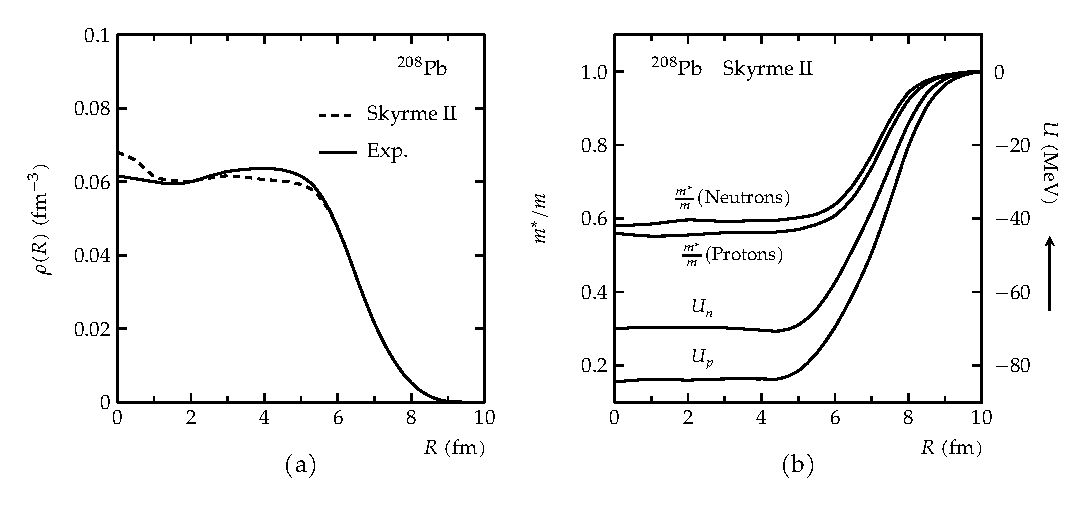
\includegraphics[width=0.85\linewidth]{pictures/5_5}
\par\end{centering}
\centering{}\caption{\label{fig:skyrme2_pb208_results}采用Skyrme II相互作用计算$^{208}\mathrm{Pb}$的Hartree-Fock结果。(a)
电荷分布；(b) 有效质量$m^{*}/m$与HF势$U(r)$（质子单粒子势未包含Coulomb项）（来自\cite{VB72}）}
\end{figure}

\begin{figure}[H]
\begin{centering}
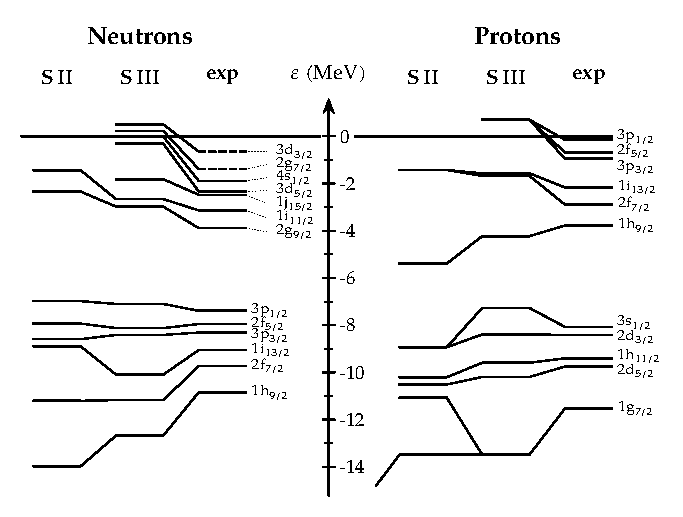
\includegraphics[width=0.8\linewidth]{pictures/5_6}
\par\end{centering}
\centering{}\caption{\label{fig:single_particle_energies_lead}铅核区实验与计算的单粒子能量。计算值由两种不同版本的Skyrme力获得。随着有效质量的增大，我们可以看到能谱的压缩（SII对应$m^{*}/m\simeq0.6$，SIII对应$\simeq0.75$）（来自\cite{BFG75}）}
\end{figure}


\section{结语\label{sec:=007ED3=008BED}}

总结本章的结果，我们可以说，第2章中所讨论的球形壳模型在此找到了微观理论基础。Hartree-Fock方法为从有效核子相互作用出发计算平均势提供了一个强有力的理论工具。为了获得与实验的定量符合，采用密度依赖的有效相互作用变得至关重要。在此框架下，我们能够非常优良地重现球形核的基态性质。在大多数情况下，计算出的单粒子能级展现出了正确的壳层排序；然而，在细节上它们与邻近奇质量核的实验单粒子激发谱之间仍存在一定偏离。

到目前为止，我们仅仅讨论了HF方法在闭壳核中的应用。事实上，只有在这些情况下，自洽平均场才能够保持球对称性。一旦在未填满的$j$壳层中放入一个或若干个粒子（开壳核HF
\cite{Ke63}），我们就必须决定原来简并的磁量子数$m$中哪一个应当被占据，从而导致轻微形变的密度分布（对于较大的$|m|$值，相对于量子化轴呈现扁椭球形变；对于较小的$|m|$值，则呈现长椭球形变）。这种形变密度在迭代的下一步中会产生形变的平均场，进而改变核芯中的单粒子波函数。通过这种方式，我们计入了由外加价粒子与其他核子相互作用所引起的关联效应。我们称这种效应为核芯的极化（polarization
of the core）。

只要我们只有单个或少数几个外加粒子，我们亦可以在球形基底中通过允许粒子-空穴（$ph$）激发的壳模型组态混合计算来处理这一相互作用。在这一图像中，价核子激发了核芯中的虚振动，我们通过粒子-振动耦合技术来处理极化效应（参见第9.3节）。

在许多实际应用中，人们往往通过将外加粒子以相等的概率$v^{2}_{m}=1/(2j+1)$均匀分布在下一个较高$j$壳层的所有$m$量子数上，从而仅以平均化的方式来考虑这种效应。在某种意义上，此时的波函数构成了一个具有球形密度分布的HFB态（参见第7章）。

原则上，只有在最高被占能级与最低未占能级之间存在明显的能隙时，平均场近似才具有充分的理论正当性。如果并非如此（例如次壳层闭合），便极易激发虚$ph$对，我们预期真实的波函数将比单一Slater行列式更加复杂{[}参见式(2.36){]}。基于这些理由，我们预期HF方法对幻数核的基态近似程度要远好于对那些偏离满壳组态若干粒子的核。这些开壳核在HF计算中表现出微小的形变，并在Fermi面附近具有许多几乎简并的能级。

如果我们继续向开壳层中添加粒子，形变就会变得越来越大。在远离满壳的开壳核中，我们会遇到强形变核（参见第3章）。在这里，HF极小值对应于一个具有显著形变的单一Slater行列式。由于平均势现在强烈地偏离球对称性，球形对称群的不可约表示（例如角动量$J$）不再是好量子数。波函数破坏了转动对称性。我们将在第3章和第11章中看到，这反映了体系自发对称性破缺（spontaneous
symmetry breaking）的物理机制。为了将计算出的形变态与真实的实验室系核态建立联系，必须通过恢复对称性（例如角动量投影）来恢复原本的转动不变性（参见第11章）。

在球形幻数核与强形变核之间，存在着一大类软核（soft nuclei）或过渡核（transitional nuclei）。在这些原子核中，势能面随形变的变化极为平缓，平均场近似无法给出清晰的能量极小值。此时，核体系呈现出剧烈的形变振荡和复杂的集体激发，必须借助生成坐标法（GCM，第10章）或玻色展开方法（第9章）等超越平均场的动力学方法进行处理。

形变Hartree-Fock理论在定量描述重质量稀土区和锕系核的转动带、内禀四极矩、六角形变以及裂变位垒方面取得了巨大成功。通过引入适当的外场下拉伸约束（constrained
HF），人们能够完整地绘制出核裂变位垒曲线\cite{FQ73,FQS73}。

总之，Hartree-Fock方法不仅构成了现代微观核结构理论的基石，而且为后续各章讨论的配对关联（BCS与HFB理论，第6、7章）、简谐微振动（RPA理论，第8章）、大振幅集体运动（GCM理论，第10章）以及对称性恢复（第11章）提供了最根本的自洽平均场出发点。
